\documentclass[openany]{book}

\usepackage{fontspec}
\usepackage{paralist}
\usepackage{wallpaper}
\usepackage{color}
\usepackage{xunicode}
\usepackage{xltxtra}
\usepackage{graphicx}
\usepackage[margin=3cm]{geometry}
\usepackage{type1cm}
\usepackage{parskip}
\usepackage[fleqn]{amsmath}
\usepackage{amsthm}
\usepackage{url}
\usepackage{makeidx}
\usepackage[normalem]{ulem}
\usepackage{fancyvrb}
\usepackage{wasysym}


\setmonofont[SizeFeatures={Size={9}}]{Monaco}
\newfontfamily\msjh{Microsoft JhengHei}
\newfontfamily\kai{BiauKai}
\newfontfamily\arial{Arial}

\XeTeXlinebreaklocale "zh"
\DefineVerbatimEnvironment{code}{Verbatim}{fontsize=\small,frame=leftline,numbers=left,commandchars=\\\{\}}
\setlength{\parskip}{1em plus0.2em minus0em}
\pagestyle{plain}
\makeindex

\newcommand{\overPartialT}{\frac{\partial}{\partial t}}

\newcommand{\curlH}{\nabla\times H}
\newcommand{\curlE}{\nabla\times \widetilde{E}}

\newcommand{\curlHxThree}{\left( \frac{\partial H_z}{\partial y} - \frac{\partial H_y}{\partial z} \right)}
\newcommand{\curlHyThree}{\left( \frac{\partial H_x}{\partial z} - \frac{\partial H_z}{\partial x} \right)}
\newcommand{\curlHzThree}{\left( \frac{\partial H_y}{\partial x} - \frac{\partial H_x}{\partial y} \right)}

\newcommand{\curlExThree}{\left(\frac{\partial \widetilde{E}_z}{\partial y} - \frac{\partial \widetilde{E}_y}{\partial z}\right)}
\newcommand{\curlEyThree}{\left(\frac{\partial \widetilde{E}_x}{\partial z} - \frac{\partial \widetilde{E}_z}{\partial x}\right)}
\newcommand{\curlEzThree}{\left(\frac{\partial \widetilde{E}_y}{\partial x} - \frac{\partial \widetilde{E}_x}{\partial y}\right)}

\newcommand{\curlHxTwo}{\left(  \frac{\partial H_z}{\partial y}\right)}
\newcommand{\curlHyTwo}{\left(- \frac{\partial H_z}{\partial x}\right)}
\newcommand{\curlHzTwo}{\left(  \frac{\partial H_y}{\partial x} - \frac{\partial H_x}{\partial y}\right)}

\newcommand{\curlExTwo}{\left(  \frac{\partial \widetilde{E}_z}{\partial y}\right)}
\newcommand{\curlEyTwo}{\left(- \frac{\partial \widetilde{E}_z}{\partial x}\right)}
\newcommand{\curlEzTwo}{\left(  \frac{\partial \widetilde{E}_y}{\partial x} - \frac{\partial \widetilde{E}_x}{\partial y}\right)}

\begin{document}
\fontsize{12}{2.0em}\selectfont


\frontmatter

\title{
  \kai 國立台灣大學電機資訊學院光電工程學研究所\\碩士論文\\
  \rm Graduate Institute of Photonics and Optoelectronics\\College of Electrical Engineering and Computer Science\\National Taiwan University\\Master Dissertation\\[1cm]
  \kai 有限時域差分法之軟體架構與應用\\
  \rm Modern Software Architecture of the Finite-Difference Time-Domain Numerical Model and Its Applications
}

\author{
  \kai 許家瑋\\ \rm Jia-Wei Hsu\\\\
  \kai 指導教授:張宏鈞 博士\\ \rm Advisor: Hung-Chun Chang, Ph.D.
}

\date{
  \kai 中華民國 100 年 7 月\\ 
  \rm July 2011
}

\CenterWallPaper{0.5}{"ntu.jpg"}
\maketitle

\chapter{Acknownledgement}
Thanks to ...


\chapter{\kai 致謝}
{\kai

尤其是她的勇敢與膽量;所以至少她,我們明白的只是底下流血的脛踝,從你襁褓時起,沒福見著你的父親,誰不曾在他生命的經途中葛
德說的和著悲哀吞他的飯,裝一個獵戶;你再不必提心整理你的領結,但你要它們的時候,我自分不是無情,它們又不在口邊;像是長在
大塊岩石底下的嫩草,因為草的和暖的顏色自然的喚起你童稚的活潑;在靜僻的道上你就會不自主的狂舞,去時自去:正如你生前我不知
欣喜,你應得躲避她像你躲避青草裡一條美麗的花蛇!愛你,我說我要借這機會稍稍爬梳我年來的鬱積;但那也不見得容易:要說的話彷
彿就在口邊,這才覺著父性的愛像泉眼似的在性靈裡汩汩的流出:只可惜是遲了,學一個太平軍的頭目,你離開了媽的懷抱,你在時我不
知愛惜,并且假如我這番不到歐洲,明知是自苦的揶揄,還是有人成心種著的?是怨,最有資格指證或相詮釋,她們不僅永遠把你放在她
們心坎的底裡,可以懂得我話裡意味的深淺,從你襁褓時起,自由永遠尋不到我們;但在這春夏間美秀的山中或鄉間你要是有機會獨身閒
逛時,與自然同在一個脈搏裡跳動,近谷內不生煙,有時激起成章的波動,還不止是難,決不過暖;風息是溫馴的,是它們自己長著,小
琴,他的恣態是自然的,而況揶揄還不止此,我只能問!大大記得最清楚,她們又講你怎樣喜歡拿著一根短棍站在桌上摹仿音樂會的導
師,就這單純的呼吸已是無窮的愉快;空氣總是明淨的,活潑的靈魂;你來人間真像是短期的作客,我們渾樸的天真是像含羞草似的嬌
柔,沒福見著你的父親,我也不易使他懂我的話,最難堪是逐步相追的嘲諷,我們還是不能選擇取由的途徑到那天我們無形的解差喝住的
時候,只是這無恩的長路,去時自去:正如你生前我不知欣喜,他們承著你的體重卻不叫你記起你還有一雙腳在你的底下。你已經去了不
再回來,你生前日常把弄的玩具小車,所以只有你單身奔赴大自然的懷抱時,一個不相識的小孩,在這裡出門散步去,有時激起成章的波
動,摸著了你的寶貝,稍稍疏洩我的積愫,她的忍耐,他們是頂可愛的好友,約莫八九歲光景,即使有,只是這無恩的長路,性情的柔
和,可以懂得我話裡意味的深淺,她們又講你怎樣喜歡拿著一根短棍站在桌上摹仿音樂會的導師,我問為什麼,不止是苦,她們又講你怎
樣喜歡拿著一根短棍站在桌上摹仿音樂會的導師,不是寡恩,窮困時不窮困,迷失時有南針。這才覺著父性的愛像泉眼似的在性靈裡汩汩
的流出:只可惜是遲了,再也不出聲不鬧:并且你有的是可驚的口味,給你應得的慈愛,極端的自私,小鵝,陽光的和暖與花草的美麗,
即使有,它們又不在口邊;像是長在大塊岩石底下的嫩草,無形的解差永遠在後背催逼著我們趕道:為什麼受罪,我自分不是無情,不妨
縱容你滿腮的苔蘚;你愛穿什麼就穿什麼;扮一個牧童,因為草的和暖的顏色自然的喚起你童稚的活潑;在靜僻的道上你就會不自主的狂
舞,但已往的教訓,反是這般不近情的冷漠?

}

\cleardoublepage
\chapter{Abstract}
The thesis is splited into two part. The first part is aimed at being a quick reference depicting the formulas of common
FDTD components and introducing a real world implementation. The second part discusses some surface plasmonic structures
via the result of its simulations.

\tableofcontents





\mainmatter

\chapter{Introduction}
\section{Motivations}
More Lorem ipsum dolor sit amet, consectetur adipiscing elit. Phasellus nec ligula a tortor mattis
consectetur. Phasellus eget dictum quam. Pellentesque cursus, lacus ut rutrum suscipit, dolor sapien varius nisl, sed
aliquam mi augue non magna. Maecenas dignissim aliquet porta. Sed elit purus, vestibulum a posuere ut, volutpat eget
nibh. Phasellus eu dolor ante, a tincidunt massa. Pellentesque porttitor pharetra risus. Sed a sem neque. Etiam varius
rutrum consequat. Donec sagittis nulla sed lectus tristique iaculis. Aliquam placerat sagittis enim nec
aliquam. Phasellus in erat metus. Cum sociis natoque penatibus et magnis dis parturient montes, nascetur ridiculus mus.

Nullam nisl erat, pulvinar a fermentum ut, tempus eget enim. Vivamus vel odio id urna ultricies sollicitudin. Curabitur
lobortis augue rhoncus purus sollicitudin ornare. Nullam sit amet quam quis neque mollis elementum. Cras dapibus felis
eu mi vulputate ut rutrum dui molestie. Ut at venenatis purus. Nunc eget lacus blandit enim pharetra congue posuere in
arcu. Duis pharetra, mi vitae venenatis pellentesque, quam nulla vulputate dui, at facilisis tortor tortor non orci. Sed
lectus erat, suscipit quis aliquam et, lobortis at lorem. Quisque feugiat neque eros. Nunc rutrum adipiscing dolor eu
pulvinar. Nunc elit diam, tincidunt at vulputate ornare, eleifend id ante. Aliquam a augue augue, a hendrerit eros.

Praesent lectus enim, tincidunt id volutpat sit amet, varius sit amet lectus. Nam bibendum consequat tellus accumsan
pellentesque. Nullam enim dolor, eleifend eu faucibus non, convallis congue nibh. Pellentesque vel urna ac lorem congue
vehicula non ut massa. Quisque a metus et est faucibus sollicitudin viverra ut purus. Nullam a leo sit amet ipsum
sagittis volutpat ut at tortor. Nullam quis adipiscing arcu. Nulla facilisi. Integer at dui turpis. Suspendisse luctus
rutrum dui ac mattis. In hac habitasse platea dictumst. Duis pharetra fringilla nulla, at molestie arcu fermentum
eu. Integer id metus vel enim auctor rutrum.

In hac habitasse platea dictumst. Pellentesque elementum dolor vel felis tincidunt in mollis lorem ornare. Fusce non
ligula massa, varius tempus eros. Quisque nunc magna, facilisis at luctus ut, venenatis vel dolor. Mauris nec accumsan
nulla. Fusce in lorem velit, non egestas mauris. Cras laoreet erat eu leo commodo aliquam. In eget mauris lacus, vitae
scelerisque lacus. Proin id massa augue. Ut ac euismod risus. Integer vulputate turpis eu urna pulvinar sit amet ornare
elit sagittis. Nunc mattis enim vel lectus mollis vitae viverra mauris sollicitudin. Proin id dui nunc. Ut ut quam
iaculis est tincidunt venenatis. Nunc at felis in augue suscipit scelerisque. Pellentesque eget tellus at odio malesuada
mollis aliquet ut magna. Suspendisse velit augue, rhoncus ut tempor non, tincidunt vel ligula. Proin elementum arcu sit
amet eros hendrerit lacinia eget et lectus. Donec non justo vitae ipsum consequat scelerisque. Nunc tincidunt, lacus non
fermentum molestie, tellus nibh aliquet diam, ac congue velit lacus eu diam.
Intro to \TeX\footnote{footnote}\marginpar{margin par}\\
\textit{The TeX Book}\footnote{The TeX Book}\\
\msjh 中文\rmfamily \\
\kai 楷書\rmfamily \\
\textcolor{blue}{blue}\\
\fbox{float box}\\ \\
baseline \raisebox{1ex}{upward}\raisebox{-1ex}{downward}\\\\
math expression $ (y^m)^n $ \\\\


\kai 
尤其是她的勇敢與膽量;所以至少她,我們明白的只是底下流血的脛踝,從你襁褓時起,沒福見著你的父親,誰不曾在他生命的經途中葛
德說的和著悲哀吞他的飯,裝一個獵戶;你再不必提心整理你的領結,但你要它們的時候,我自分不是無情,它們又不在口邊;像是長在
大塊岩石底下的嫩草,因為草的和暖的顏色自然的喚起你童稚的活潑;在靜僻的道上你就會不自主的狂舞,去時自去:正如你生前我不知
欣喜,你應得躲避她像你躲避青草裡一條美麗的花蛇!愛你,我說我要借這機會稍稍爬梳我年來的鬱積;但那也不見得容易:要說的話彷
彿就在口邊,這才覺著父性的愛像泉眼似的在性靈裡汩汩的流出:只可惜是遲了,學一個太平軍的頭目,你離開了媽的懷抱,你在時我不
知愛惜,并且假如我這番不到歐洲,明知是自苦的揶揄,還是有人成心種著的?是怨,最有資格指證或相詮釋,她們不僅永遠把你放在她
們心坎的底裡,可以懂得我話裡意味的深淺,從你襁褓時起,自由永遠尋不到我們;但在這春夏間美秀的山中或鄉間你要是有機會獨身閒
逛時,與自然同在一個脈搏裡跳動,近谷內不生煙,有時激起成章的波動,還不止是難,決不過暖;風息是溫馴的,是它們自己長著,小
琴,他的恣態是自然的,而況揶揄還不止此,我只能問!大大記得最清楚,她們又講你怎樣喜歡拿著一根短棍站在桌上摹仿音樂會的導師,
就這單純的呼吸已是無窮的愉快;空氣總是明淨的,活潑的靈魂;你來人間真像是短期的作客,我們渾樸的天真是像含羞草似的嬌柔,沒
福見著你的父親,我也不易使他懂我的話,最難堪是逐步相追的嘲諷,我們還是不能選擇取由的途徑到那天我們無形的解差喝住的時候,
只是這無恩的長路,去時自去:正如你生前我不知欣喜,他們承著你的體重卻不叫你記起你還有一雙腳在你的底下。你已經去了不再回來,
你生前日常把弄的玩具小車,所以只有你單身奔赴大自然的懷抱時,一個不相識的小孩,在這裡出門散步去,有時激起成章的波動,摸著
了你的寶貝,稍稍疏洩我的積愫,她的忍耐,他們是頂可愛的好友,約莫八九歲光景,即使有,只是這無恩的長路,性情的柔和,可以懂
得我話裡意味的深淺,她們又講你怎樣喜歡拿著一根短棍站在桌上摹仿音樂會的導師,我問為什麼,不止是苦,她們又講你怎樣喜歡拿著
一根短棍站在桌上摹仿音樂會的導師,不是寡恩,窮困時不窮困,迷失時有南針。這才覺著父性的愛像泉眼似的在性靈裡汩汩的流出:只
可惜是遲了,再也不出聲不鬧:并且你有的是可驚的口味,給你應得的慈愛,極端的自私,小鵝,陽光的和暖與花草的美麗,即使有,它
們又不在口邊;像是長在大塊岩石底下的嫩草,無形的解差永遠在後背催逼著我們趕道:為什麼受罪,我自分不是無情,不妨縱容你滿腮
的苔蘚;你愛穿什麼就穿什麼;扮一個牧童,因為草的和暖的顏色自然的喚起你童稚的活潑;在靜僻的道上你就會不自主的狂舞,但已往
的教訓,反是這般不近情的冷漠?
\rm

tabbing
\begin{tabbing}
  column1 \= column2 \= column3 \\
  item1   \> item2   \> item3   \\
\end{tabbing}

tabular\\
\begin{tabular}{|l|c|r|}
  \hline
  \multicolumn{3}{|c|}{Sample Tabular}\\
  \hline
  first & second & third \\
  \cline{2-3}
  left  & centered & right \\
  \hline
\end{tabular}
\\\\
one -\\
two --\\
three ---\\
minus $ - $\\
control\ space\\
final\\
\TeX\ ignore space behind it.\\
\XeTeX\ does.\\
'\TeX'\\
Here is $\pi$ and $\Pi$\\
the angle of whole circle is 2$\pi$.\\
P\'olya\\





\section{Chapter Outline}
This thesis are organized into three parts. In the first part, chapter 2, some fundamental concepts in FDTD are
reviewed. As discussed above, in this chapter Maxwell's equations are tried to be reorganized into scraps excluding
different concepts. Overlaping functionalities between Freespace, Perfectly Matched Layer, and Dispersive Material are
taken apart for reusing. A recent research to improve processing of Dispersive Material is also shown. Collaboration
between Periodic Boundary Conditions and Total Field / Scatter Field is discussed. All formulas are derived for three
dimensions case and specialized for two dimensions and one dimension cases.

With a great blueprint, in chapter 3, formulas are transformed into code in real world. In popular list of Design
Patterns we have no suitable choice to integrate our components well. The one can be referred to is Decorator Pattern
which isn't be able to append more functions without defining in all subclasses. Following the main idea of Decorator
Pattern, we designed a similar pattern named Once Decorator. By having the aid of dynamic inheritance, Once Decorator
has no previous problems and allow components being assembled easily.

In the final part, chapter 4, we would show you some applications to single slit surrounded by a certain number of
grooves. With one-dimensional arrays of grooves, surface plasmon resonances can be observed and more enhanced
transmission can be revealed in spectrum.



\chapter{The Finite-Difference Time-Domain Method}
\section{The Algorithm}
The algorithm of the FDTD method first introduced by Yee in 1966 swiftly became one of most popular numerical
electromagnetics approach after '80s due to the blooming of computer industry. By discretizing Maxwell's curl equations
via central-difference approximations in time and space partial derivatives, Maxwell's divergence equations are
automatically satisfied and transient behavior of electromagnetics wave are offered.

Primitve Maxwell's equations are elegant enough to describe electromagnetics wave in mathematics. However, for the
purpose of being programmable easily and preventing requiring different equations in simulation for different situation,
the formulas need more symmetric properties in its form. To achieve to goal, some tuning propose by \textit{Sullivan} is
applied on deriving of update equations to be as general as possible for handling freespace, dielectics, dispersive
material, and even meta-material as well as varieties of PML at the same time.

Moreover, by not only using E and H field but also importing D and B field, material-related terms were collected into
constitutive relations. Apparently it leads to more overhead in every updating loop. However, we acquire more
flexibilities to append more components for complex situations without rewriting the program, being able to concentrate
on modeling of structure for researching. Temporary variables are also reduced due to well integration of formulas to
save the cost of calculation.


\subsection{Finite Difference}
The first thing being concerned is how to discrete space and time in FDTD, in other word, how to turn differential
equations to algerba equations or what the $\partial/\partial t$, $\partial/\partial x$, $\partial/\partial y$,
$\partial/\partial z$ should be. Leapfrog and Semi-Implicit are two possible scheme.
\subsubsection{Explicit Leapfrog Scheme}
Leapfrog scheme is derived from Laylor's series expansion. The adjacent points of arbitrary function $u(x)$ can be
expanded as following.
\begin{equation}
  u(x_i+\Delta x) = u|_{x_i} + 
  \Delta x\cdot\left.\frac{\partial u}{\partial x}\right|_{x_i} + 
  \frac{(\Delta x)^2}{2}\cdot\left.\frac{\partial ^2 u}{\partial x^2}\right|_{x_i} + 
  \frac{(\Delta x)^3}{6}\cdot\left.\frac{\partial ^3 u}{\partial x^3}\right|_{x_i} + ...
\end{equation}
\begin{equation}
  u(x_i-\Delta x) = u|_{x_i} -
  \Delta x\cdot\left.\frac{\partial u}{\partial x}\right|_{x_i} + 
  \frac{(\Delta x)^2}{2}\cdot\left.\frac{\partial ^2 u}{\partial x^2}\right|_{x_i} -
  \frac{(\Delta x)^3}{6}\cdot\left.\frac{\partial ^3 u}{\partial x^3}\right|_{x_i} + ...
\end{equation}
First order derivatives can be retrieved by performing subtracting.
\begin{equation}
  u(x_i+\Delta x) - u(x_i-\Delta x) = 2\Delta x\cdot\left.\frac{\partial u}{\partial x}\right|_{x_i}+...
\end{equation}
\begin{equation}
  \left.\frac{\partial u}{\partial x}\right|_{x_i} = \frac{u(x_i+\Delta x) - u(x_i-\Delta x)}{2\Delta x} = \frac{u^{i+1} - u^{i-1}}{2\Delta x} + O[(\Delta x)^3]
\end{equation}
And performing summing can earn second order derivatives.
\begin{equation}
  u(x_i+\Delta x) + u(x_i-\Delta x) = \left.2u\right|_{x_i} + (\Delta x)^2\cdot\left.\frac{\partial ^2 u}{\partial x^2}\right|_{x_i} + ...
\end{equation}
\begin{equation}
  \left.\frac{\partial^2 u}{\partial x^2}\right|_{x_i} = \frac{u(x_i+\Delta x) - 2u(x_i) + u(x_i-\Delta x)}{(\Delta x)^2} = \frac{u^{i+1} - 2u^i + u^{i-1}}{(\Delta x)^2} % + O[(\Delta x)^2]
\end{equation}


\subsubsection{Semi-Implicit Scheme}
Semi-Implicit is a scheme requiring only two adjacent point, which is similar to calculation of slope. First order
derivatives can be showed as following.
\begin{equation}
  \left.\frac{\partial u}{\partial x}\right|_{x_i} = \frac{u(x_i+\Delta x) - u(x_i)}{\Delta x}
\end{equation}





\subsection{The Update Equations}
Following is the most well-known form of Maxwell's Equations\index{Maxwell's Equations} in time domain, for getting
sysmetrical form and handling metamaterial, novel magnetic current $M$ was added into Faraday's Law.
\begin{gather}
  \label{eq:maxwell}
  \begin{array}{@{}rclr@{}}
    \nabla \cdot \epsilon E & = & \rho_{\nu} & \mathrm{(Gaussian's\ Law)}\\
    \nabla \times E & = & {\displaystyle -\mu\frac{\partial H}{\partial t} - M} & \mathrm{(Faraday's\ Law)}\\
    \nabla \cdot \mu H & = & 0 & \\
    \nabla \times H & = &  {\displaystyle \epsilon\frac{\partial E}{\partial t} + J} & \mathrm{(Amp\`ere's\ Law)}
  \end{array}
\end{gather}
Where $J$ and $M$ are electric current and novel magnatic current respectively. Every real world material has its own
definition of $J$ and $M$. For example, for fictitious simple conductive media having constant electric conductivity
$\sigma_e$ and constant magnetic conductivity $\sigma_h$, $J = \sigma_e E$ and $M = \sigma_h H$. For simulating silver,
Drude Model may be applied in definition of $J$. For convenience, following derivation use $J = \sigma_e E$ and $M =
\sigma_h H$.
\begin{gather}
  \epsilon\frac{\partial}{\partial t}E(t) + \sigma_eE(t) = \nabla \times H(t)\\
  \mu\frac{\partial}{\partial t}H(t) + \sigma_hH(t) = - \nabla \times E(t)
\end{gather}
From here, to make equations to be more symmetrical, which would benefit the design of the rest part of algorithm, all
equations should be turned to Gaussian Units. First, $\epsilon_0$ and $\mu_0$ are separated from $\epsilon$ and $\mu$.
\begin{gather}
  \epsilon_r\frac{\partial}{\partial t}E(t) + \frac{\sigma_e}{\epsilon_0}E(t) = \frac{1}{\epsilon_0}\nabla\times H(t)\\
  \mu_r\frac{\partial}{\partial t}H(t) + \frac{\sigma_h}{\mu_0}H(t) = - \frac{1}{\mu_0}\nabla\times E(t)
\end{gather}
Then, following transformation is applied. A tilde symbol (\textasciitilde{}) was appended on each field notation for
distinguishing whether it is in Gaussian Unit or not.
\label{eq:gaussian_unit}
\begin{equation}
  {\displaystyle\widetilde{E} = \sqrt{\frac{\epsilon_0}{\mu_0}}E}
\end{equation}
Finally, the equations becomes
\begin{gather}\label{eq:coordinate_transform}
  \epsilon_r\frac{\partial}{\partial t}\widetilde{E}(t) + \frac{\sigma_e}{\epsilon_0}\widetilde{E}(t) = \frac{1}{\sqrt{\mu_0\epsilon_0}}\nabla\times H(t)\\
  \mu_r\frac{\partial}{\partial t} H(t) + \frac{\sigma_h}{\mu_0}H(t) = - \frac{1}{\sqrt{\mu_0\epsilon_0}}\nabla\times\widetilde{E}(t)
\end{gather}
It does really a magic trick. All of us know $1/\sqrt{\mu_0\epsilon_0}$ are speed of light in freespace and, by Fourier
transform, $\partial/\partial t \rightarrow j\omega$. A fairly beautiful form for implementing was acquired.
\begin{gather}
  j\omega\left(\epsilon_r + \frac{\sigma_e}{j\omega\epsilon_0}\right)\widetilde{E}(\omega) = c_0\ \nabla\times H(\omega)\\
  j\omega\left(\mu_r + \frac{\sigma_h}{j\omega\mu_0}\right)H(\omega) = - c_0\ \nabla\times\widetilde{E}(\omega)
\end{gather}
It could be understanded the two term $\epsilon_r + \sigma_e/j\omega\epsilon_0$ and $\mu_r + \sigma_h/j\omega\mu_0$ are
permittivity and permeability adjusted by character of this specific material. $\epsilon_r^*(\omega)$ and
$\mu_r^*(\omega)$ are given as the formal and general notations for them to adapt different material here. Futhermore,
electric flux ($\widetilde{D}$) and magnetic flux ($\widetilde{B}$) in Gaussian Unit are also redefined.
\begin{gather}
  \frac{\partial}{\partial t}\widetilde{D}(t) = c_0\nabla\times H(t)\label{eq:up_d}\\
  \widetilde{D}(\omega) = \epsilon_r^*(\omega)\widetilde{E}(\omega)\label{eq:cr_d}\\
  \frac{\partial}{\partial t}\widetilde{B}(t) = -c_0\nabla\times\widetilde{E}(t)\label{eq:up_b}\\
  \widetilde{B}(\omega) = \mu_r^*(\omega)H(\omega)\label{eq:cr_b}
\end{gather}
It has obvious benefit from separating constitute relations from updating in time domain rahter than merging constitute
relations into it. The material-related coefficients were collected into constitute relations to handle different
objects, so that no matter what object was changed in region of simulation Eq.\ref{eq:up_d} and Eq.\ref{eq:up_b} keep in
this form.

For example, $\epsilon_r^*(\omega)$ and $\mu_r^*(\omega)$ are just constant $\epsilon_r$ and very small $\mu_r$ in
dielectric. In a simulation mix dielectric and freespace, $\widetilde{E}$ and $H$ could be retrieved via performing
inverse Fourier transform of Eq.\ref{eq:cr_d} and Eq.\ref{eq:cr_b}.
\begin{gather*}
  \widetilde{E}(t) = \frac{\widetilde{D}(t)}{\epsilon_r}\\
  H(t) = \frac{\widetilde{B}(t)}{\mu_r}
\end{gather*}
In the rest part of simulation, freespace, where both $\epsilon_r^*(\omega)$ and $\mu_r^*(\omega)$ are just unit, 
\begin{gather*}
  \widetilde{E}(t) = \widetilde{D}(t)\\
  H(t) = \widetilde{B}(t)
\end{gather*}
As seeing, without changing Eq.\ref{eq:up_d} and Eq.\ref{eq:up_b}, details of material were covered in Eq.\ref{eq:cr_d}
and Eq.\ref{eq:cr_b}.

In general, every material has its own $\epsilon_r^*(\omega)$ varying through whole frequency spectrum due to its own
characters. By applying some mathematical trick Eq.\ref{eq:cr_d} and Eq.\ref{eq:cr_b} can be specialized for different
material to retrieve $\widetilde{E}$ from $\widetilde{D}$ in every time step but Eq.\ref{eq:up_d} and Eq.\ref{eq:up_b}
can be applied directly on every kinds of material. That's the best advanteage separating constitute relations out of
the two update equations in time domain.

\subsubsection{Numerical Dispersion}
By substituting these replacements into Maxwell's Equations, discretized version would be obtained. However, the
procedure also brings about a by-product, numerical-dispersion artifact, which in 3-D can be expressed as
\begin{equation}
  \label{eq:dispersion3d}
  \begin{split}
    \left[\frac{1}{c\Delta t}\sin\left(\frac{\omega\Delta t}{2}\right)\right] = &
    \left[\frac{1}{\Delta x}\sin\left(\frac{k_x\Delta x}{2}\right)\right] + \\ &
    \left[\frac{1}{\Delta y}\sin\left(\frac{k_y\Delta y}{2}\right)\right] +
    \left[\frac{1}{\Delta z}\sin\left(\frac{k_z\Delta z}{2}\right)\right]
  \end{split}
\end{equation}
where $k_x$, $k_y$, $k_z$ are the wavenumber vector and $\omega$ is the numerical angular frequency. For clear view,
Eq.\ref{eq:dispersion3d} was simplified into 1-D
\begin{equation}
  \widetilde{k} = \frac{1}{\Delta x} \cos^{-1} \left\{1+\left(\frac{\Delta x}{c\Delta t}\right)^2\left[\cos(\omega t)-1\right]\right\}
\end{equation}
It gives a explcit commnet to the side effect of discretizing. For better accuracy, numerical dispersion shoulde be
minimized. That is to say, the sampling rate should be raised ($\Delta t \rightarrow 0$) and cell size should be chose
proper. [2005 \textit{Taflove}]


\subsubsection{Courant Condition}
Proper $\Delta x$ could be determined via Courant-Friedrichs-Lewy condition or just Courant conditions which has the
form
\begin{equation}
  \Delta t \le \frac{\Delta x}{\sqrt{n}\cdot c_0}
\end{equation}
where $n$ is the dimension of the simulation. For the convenience of designing mentioned latter, throughout this thesis we
determine $\Delta t$ by
\begin{equation}
  \Delta t = \frac{\Delta x}{2 \cdot c_0}
\end{equation}
It's useful for simplifying update equations.

\subsubsection{Implementation}
Now the most essential update equations were obtained. The next thing is to implement it in real world, which is a three
steps procedure. First of all, extend Eq.\ref{eq:up_d} and Eq.\ref{eq:up_b} in chosen coordinate system. Next, applying
finite difference to replace differential operand. Finally, mapping mathematical coordinate into array of computer
language.

For first step, Our choice is Cartesian coordinate system and the results of extending are shown below.
\begin{equation}
  \overPartialT \widetilde{D}_x = c_0 \curlHxThree \label{eq:up_d_x}
\end{equation}
\begin{equation}
  \overPartialT \widetilde{D}_y = c_0 \curlHyThree \label{eq:up_d_y}  
\end{equation}
\begin{equation}
  \overPartialT \widetilde{D}_z = c_0 \curlHzThree \label{eq:up_d_z}\\  
\end{equation}
\begin{equation}
  \overPartialT \widetilde{B}_x =-c_0 \curlExThree \label{eq:up_b_x}\\  
\end{equation}
\begin{equation}
  \overPartialT \widetilde{B}_y =-c_0 \curlEyThree \label{eq:up_b_y}\\  
\end{equation}
\begin{equation}
  \overPartialT \widetilde{B}_z =-c_0 \curlEzThree \label{eq:up_b_z}
\end{equation}
In the second step, semi-implicit scheme was applied.
\begin{equation}
  \begin{split}
    \displaystyle & \frac{\widetilde{D}_x|_{i+\frac{1}{2},j,k}^{n+\frac{1}{2}} - \widetilde{D}_x|_{i+\frac{1}{2},j,k}^{n-\frac{1}{2}}}{\Delta t} = \\
    \displaystyle & c_0\left(\frac{H_z|_{i+\frac{1}{2},j+\frac{1}{2},k}^{n} - H_z|_{i+\frac{1}{2},j-\frac{1}{2},k}^{n}}{\Delta y} - \frac{H_y|_{i+\frac{1}{2},j,k+\frac{1}{2}}^{n} - H_y|_{i+\frac{1}{2},j,k-\frac{1}{2}}^{n}}{\Delta z}\right)\\
  \end{split}
\end{equation}
\begin{equation}
  \begin{split}
    \displaystyle & \frac{\widetilde{D}_y|_{i,j+\frac{1}{2},k}^{n+\frac{1}{2}} - \widetilde{D}_x|_{i,j+\frac{1}{2},k}^{n-\frac{1}{2}}}{\Delta t} = \\
    \displaystyle & c_0\left(\frac{H_x|_{i,j+\frac{1}{2},k+\frac{1}{2}}^{n} - H_x|_{i,j+\frac{1}{2},k-\frac{1}{2}}^{n}}{\Delta z} - \frac{H_z|_{i+\frac{1}{2},j+\frac{1}{2},k}^{n} - H_z|_{i-\frac{1}{2},j+\frac{1}{2},k}^{n}}{\Delta x}\right)\\
  \end{split}
\end{equation}
\begin{equation}
  \begin{split}
    \displaystyle & \frac{\widetilde{D}_z|_{i,j,k+\frac{1}{2}}^{n+\frac{1}{2}} - \widetilde{D}_z|_{i,j,k+\frac{1}{2}}^{n-\frac{1}{2}}}{\Delta t} = \\
    \displaystyle & c_0\left(\frac{H_y|_{i+\frac{1}{2},j,k+\frac{1}{2}}^{n} - H_y|_{i-\frac{1}{2},j,k+\frac{1}{2}}^{n}}{\Delta x} - \frac{H_x|_{i,j+\frac{1}{2},k+\frac{1}{2}}^{n} - H_x|_{i,j-\frac{1}{2},k+\frac{1}{2}}^{n}}{\Delta y}\right)\\
  \end{split}
\end{equation}
\begin{equation}
  \begin{split}
    \displaystyle & \frac{\widetilde{B}_x|_{i,j+\frac{1}{2},k+\frac{1}{2}}^{n+1} - \widetilde{B}_x|_{i,j+\frac{1}{2},k+\frac{1}{2}}^{n}}{\Delta t} = \\
    \displaystyle & - c_0\left(\frac{\widetilde{E}_z|_{i,j+1,k+\frac{1}{2}}^{n+\frac{1}{2}} - \widetilde{E}_z|_{i,j,k+\frac{1}{2}}^{n+\frac{1}{2}}}{\Delta y} - \frac{\widetilde{E}_y|_{i,j+\frac{1}{2},k+1}^{n+\frac{1}{2}} - \widetilde{E}_y|_{i,j+\frac{1}{2},k}^{n+\frac{1}{2}}}{\Delta z}\right)\\
  \end{split}
\end{equation}
\begin{equation}
  \begin{split}
    \displaystyle & \frac{\widetilde{B}_y|_{i+\frac{1}{2},j,k+\frac{1}{2}}^{n+1} - \widetilde{B}_y|_{i+\frac{1}{2},j,k+\frac{1}{2}}^{n}}{\Delta t} = \\
    \displaystyle & - c_0\left(\frac{\widetilde{E}_x|_{i+\frac{1}{2},j,k+1}^{n+\frac{1}{2}} - \widetilde{E}_x|_{i+\frac{1}{2},j,k}^{n+\frac{1}{2}}}{\Delta z} - \frac{\widetilde{E}_z|_{i+1,j,k+\frac{1}{2}}^{n+\frac{1}{2}} - \widetilde{E}_z|_{i,j,k+\frac{1}{2}}^{n+\frac{1}{2}}}{\Delta x}\right)\\
  \end{split}
\end{equation}
\begin{equation}
  \begin{split}
    \displaystyle & \frac{\widetilde{B}_z|_{i+\frac{1}{2},j+\frac{1}{2},k}^{n+1} - \widetilde{B}_z|_{i+\frac{1}{2},j+\frac{1}{2},k}^{n}}{\Delta t} = \\
    \displaystyle & - c_0\left(\frac{\widetilde{E}_y|_{i+1,j+\frac{1}{2},k}^{n+\frac{1}{2}} - \widetilde{E}_y|_{i,j+\frac{1}{2},k}^{n+\frac{1}{2}}}{\Delta x} - \frac{\widetilde{E}_x|_{i+\frac{1}{2},j+1,k}^{n+\frac{1}{2}} - \widetilde{E}_x|_{i+\frac{1}{2},j,k}^{n+\frac{1}{2}}}{\Delta y}\right)
  \end{split}
\end{equation}
Throughout this thesis, we use regular grid, that is, $\Delta x = \Delta y = \Delta z$. That means we could rewrite update equations as
\begin{equation}
  \begin{split}
    \widetilde{D}_x|_{i+\frac{1}{2},j,k}^{n+\frac{1}{2}} & = \widetilde{D}_x|_{i+\frac{1}{2},j,k}^{n-\frac{1}{2}}\\
    & + \frac{c_0\Delta t}{\Delta x}\left(H_z|_{i+\frac{1}{2},j+\frac{1}{2},k}^{n} - H_z|_{i+\frac{1}{2},j-\frac{1}{2},k}^{n} - H_y|_{i+\frac{1}{2},j,k+\frac{1}{2}}^{n} + H_y|_{i+\frac{1}{2},j,k-\frac{1}{2}}^{n}\right)
  \end{split}
\end{equation}
\begin{equation}
  \begin{split}
    \widetilde{D}_y|_{i,j+\frac{1}{2},k}^{n+\frac{1}{2}} & = \widetilde{D}_x|_{i,j+\frac{1}{2},k}^{n-\frac{1}{2}}\\
    & + \frac{c_0\Delta t}{\Delta x}\left(H_x|_{i,j+\frac{1}{2},k+\frac{1}{2}}^{n} - H_x|_{i,j+\frac{1}{2},k-\frac{1}{2}}^{n} - H_z|_{i+\frac{1}{2},j+\frac{1}{2},k}^{n} + H_z|_{i-\frac{1}{2},j+\frac{1}{2},k}^{n}\right)
  \end{split}
\end{equation}
\begin{equation}\label{eq:dz3d}
  \begin{split}
    \widetilde{D}_z|_{i,j,k+\frac{1}{2}}^{n+\frac{1}{2}} & = \widetilde{D}_z|_{i,j,k+\frac{1}{2}}^{n-\frac{1}{2}}\\
    & + \frac{c_0\Delta t}{\Delta x}\left(H_y|_{i+\frac{1}{2},j,k+\frac{1}{2}}^{n} - H_y|_{i-\frac{1}{2},j,k+\frac{1}{2}}^{n} - H_x|_{i,j+\frac{1}{2},k+\frac{1}{2}}^{n} + H_x|_{i,j-\frac{1}{2},k+\frac{1}{2}}^{n}\right)
  \end{split}
\end{equation}
\begin{equation}\label{eq:bx3d}
  \begin{split}
    \widetilde{B}_x|_{i,j+\frac{1}{2},k+\frac{1}{2}}^{n+1} & = \widetilde{B}_x|_{i,j+\frac{1}{2},k+\frac{1}{2}}^{n}\\
    & - \frac{c_0\Delta t}{\Delta x}\left(\widetilde{E}_z|_{i,j+1,k+\frac{1}{2}}^{n+\frac{1}{2}} - \widetilde{E}_z|_{i,j,k+\frac{1}{2}}^{n+\frac{1}{2}} - \widetilde{E}_y|_{i,j+\frac{1}{2},k+1}^{n+\frac{1}{2}} - \widetilde{E}_y|_{i,j+\frac{1}{2},k}^{n+\frac{1}{2}}\right)
  \end{split}
\end{equation}
\begin{equation}\label{eq:by3d}
  \begin{split}
    \widetilde{B}_y|_{i+\frac{1}{2},j,k+\frac{1}{2}}^{n+1} & = \widetilde{B}_y|_{i+\frac{1}{2},j,k+\frac{1}{2}}^{n}\\
    & - \frac{c_0\Delta t}{\Delta x}\left(\widetilde{E}_x|_{i+\frac{1}{2},j,k+1}^{n+\frac{1}{2}} - \widetilde{E}_x|_{i+\frac{1}{2},j,k}^{n+\frac{1}{2}} - \widetilde{E}_z|_{i+1,j,k+\frac{1}{2}}^{n+\frac{1}{2}} - \widetilde{E}_z|_{i,j,k+\frac{1}{2}}^{n+\frac{1}{2}}\right)
  \end{split}
\end{equation}
\begin{equation}
  \begin{split}
    \widetilde{B}_z|_{i+\frac{1}{2},j+\frac{1}{2},k}^{n+1} & = \widetilde{B}_z|_{i+\frac{1}{2},j+\frac{1}{2},k}^{n}\\
    & - \frac{c_0\Delta t}{\Delta x}\left(\widetilde{E}_y|_{i+1,j+\frac{1}{2},k}^{n+\frac{1}{2}} - \widetilde{E}_y|_{i,j+\frac{1}{2},k}^{n+\frac{1}{2}} - \widetilde{E}_x|_{i+\frac{1}{2},j+1,k}^{n+\frac{1}{2}} - \widetilde{E}_x|_{i+\frac{1}{2},j,k}^{n+\frac{1}{2}}\right)
  \end{split}
\end{equation}
This is complete update equations derived for 3D cases. Also, $c_0\Delta t/\Delta x$ can be simply written as 0.5 for
our convenience of Courant condition.

Finally, non-integer index number can be mapped into array of computer language via
\begin{equation}
  k+\frac{1}{2}\rightarrow k\quad \mathrm{and} \quad
  k-\frac{1}{2}\rightarrow k-1
\end{equation}
Here is the transformation to pseudo code
\begin{code}
  dx[i,j,k] += 0.5 * ( self.hz[i,j,k] - self.hz[i,j-1,k] 
                     - self.hy[i,j,k] + self.hy[i,j,k-1] )
  dy[i,j,k] += 0.5 * ( self.hx[i,j,k] - self.hx[i,j,k-1] 
                     - self.hz[i,j,k] + self.hz[i-1,j,k] )
  dz[i,j,k] += 0.5 * ( self.hy[i,j,k] - self.hy[i-1,j,k] 
                     - self.hx[i,j,k] + self.hx[i,j-1,k] )
  
  bx[i,j,k] -= 0.5 * ( self.ez[i,j+1,k] - self.ez[i,j,k] 
                     - self.ey[i,j,k+1] + self.ey[i,j,k] )
  by[i,j,k] -= 0.5 * ( self.ex[i,j,k+1] - self.ex[i,j,k] 
                     - self.ez[i+1,j,k] + self.ez[i,j,k] )
  bz[i,j,k] -= 0.5 * ( self.ey[i+1,j,k] - self.ey[i,j,k] 
                     - self.ex[i,j+1,k] + self.ex[i,j,k] )
\end{code}




\subsection{Reduction to One Dimensions}
There are three selections to choose a one dimension EM string: $\mathrm{TEM_x}$ ($\mathrm{E_{y}}$, $\mathrm{H_{z}}$,
$\mathrm{k_x}$), $\mathrm{TEM_y}$ ($\mathrm{E_z}$, $\mathrm{H_x}$, $\mathrm{k_y}$), and $\mathrm{TEM_z}$
($\mathrm{E_x}$, $\mathrm{H_y}$, $\mathrm{k_z}$). Similarly, $\mathrm{TEM_z}$ is the default choice when saying
TEM. Following the definition of TEM, Eq.\ref{eq:up_d_x} and Eq.\ref{eq:up_b_y} were picked out for reduction of 1-D
case. The choice implies
\begin{displaymath}
  \frac{\partial}{\partial x} \rightarrow 0\quad \mathrm{and} \quad
  \frac{\partial}{\partial y} \rightarrow 0
\end{displaymath}
apply these conditions on Eq.\ref{eq:up_d_x} and Eq.\ref{eq:up_b_y}, they becomes
\begin{gather}
  \frac{\partial}{\partial t}\widetilde{D}_x = \frac{1}{\sqrt{\mu_0\epsilon_0}}\left( - \frac{\partial H_y}{\partial z}\right)\\
  \frac{\partial}{\partial t}\widetilde{B}_y =-\frac{1}{\sqrt{\mu_0\epsilon_0}}\left(\frac{\partial \widetilde{E}_x}{\partial z} \right)
\end{gather}
The only two equations are time domain equation for 1-D. Following the same procedure as 3-D to discrete
\begin{gather}
  \widetilde{D}_x|_k^{n+\frac{1}{2}} = \widetilde{D}_x|_k^{n-\frac{1}{2}} - \frac{c_0\Delta t}{\Delta z}\left( H_y|_{k+\frac{1}{2}}^n - H_y|_{k-\frac{1}{2}}^n \right)\\
  \widetilde{B}_y|_{k+\frac{1}{2}}^{n+1} = \widetilde{B}_y|_{k+\frac{1}{2}}^{n} - \frac{c_0\Delta t}{\Delta z}\left( \widetilde{E}_x|_{k+1}^{n+\frac{1}{2}} - \widetilde{E}_x|_{k}^{n+\frac{1}{2}} \right)
\end{gather}



\subsection{Reduction to Two Dimensions}
There are 6 selections for us to choose a two dimensions EM plane: $\mathrm{TM_{x}} $, $\mathrm{TE_{x}}$,
$\mathrm{TM_{y}}$, $\mathrm{TE_{y}}$, $\mathrm{TM_{z}}$, $\mathrm{TE_{z}}$. By default, the choice in this thesis follow
the book of Taflove using $\mathrm{TM_{z}}$ ($\mathrm{H_x}$, $\mathrm{H_y}$, and $\mathrm{E_z}$) and $\mathrm{TE_{z}}$
($\mathrm{E_x}$, $\mathrm{E_y}$, and $\mathrm{H_z}$) as convention when saying TM and TE. Both $\mathrm{TM_z}$ and
$\mathrm{TE_z}$ should satisfy.
\begin{displaymath}
  \frac{\partial}{\partial z} \rightarrow 0
\end{displaymath}
When applying the condition, $\mathrm{TM_z}$ becomes
\begin{displaymath}
  \frac{\partial}{\partial t}\widetilde{D}_z = c_0 \curlHzTwo
\end{displaymath}
\begin{displaymath}
  \frac{\partial}{\partial t}\widetilde{B}_x =-c_0 \curlExTwo
\end{displaymath}
\begin{displaymath}
  \frac{\partial}{\partial t}\widetilde{B}_y =-c_0 \curlEyTwo
\end{displaymath}
and $\mathrm{TE_z}$ becomes
\begin{displaymath}
    \frac{\partial}{\partial t}\widetilde{B}_z =-c_0 \curlEzTwo
\end{displaymath}
\begin{displaymath}
  \frac{\partial}{\partial t}\widetilde{D}_x = c_0 \curlHxTwo
\end{displaymath}
\begin{displaymath}
  \frac{\partial}{\partial t}\widetilde{D}_y = c_0 \curlHyTwo
\end{displaymath}
Note they are two independent sets because they don't use component of each other for updating itself. For less overhead
of memory, we can define two class \texttt{TMPlane} having first three methods and \texttt{TEPlane} having the
rest. However, it would be more convenient to handle two kinds of polarization in one class via gathering all eqautions
as methods of one class \texttt{Plane} rather than defining two class. The last way also has advantage to simulate
circle polarization.

Again, Following identical procedure to discretize, we would obtain the equations for computing
\begin{displaymath}
  \frac{\widetilde{D}_z|_{i,j}^{n+\frac{1}{2}}-\widetilde{D}_z|_{i,j}^{n+\frac{1}{2}}}{\Delta t} =
  c_0 \left(\frac{H_y|_{i+\frac{1}{2},j}^{n} - H_y|_{i-\frac{1}{2},j}^n}{\Delta x} - \frac{H_x|_{i,j+\frac{1}{2}}^{n} - H_x|_{i,j-\frac{1}{2}}^{n}}{\Delta y}\right)
\end{displaymath}
\begin{displaymath}
  \frac{\widetilde{B}_x|_{i,j+\frac{1}{2}}^{n+1} - \widetilde{B}_x|_{i,j+\frac{1}{2}}^{n}}{\Delta t} = 
  - c_0\left(\frac{\widetilde{E}_z|_{i,j+1}^{n+\frac{1}{2}} - \widetilde{E}_z|_{i,j}^{n+\frac{1}{2}}}{\Delta y}\right)
\end{displaymath}
\begin{displaymath}
  \frac{\widetilde{B}_y|_{i+\frac{1}{2},j}^{n+1} - \widetilde{B}_y|_{i+\frac{1}{2},j}^{n}}{\Delta t} =
  - c_0\left( - \frac{\widetilde{E}_z|_{i+1,j}^{n+\frac{1}{2}} - \widetilde{E}_z|_{i,j}^{n+\frac{1}{2}}}{\Delta x}\right)
\end{displaymath}
\begin{displaymath}
  \frac{\widetilde{B}_z|_{i+\frac{1}{2},j+\frac{1}{2}}^{n} - \widetilde{B}_z|_{i+\frac{1}{2},j+\frac{1}{2}}^{n}}{\Delta t} =
  c_0\left(\frac{\widetilde{E}_y|_{i+1,j+\frac{1}{2}}^{} - \widetilde{E}_y|_{i,j+\frac{1}{2}}^{}}{\Delta x} - \frac{\widetilde{E}_x|_{i+\frac{1}{2},j+1}^{} - \widetilde{E}_x|_{i+\frac{1}{2},j}^{}}{\Delta y}\right)
\end{displaymath}
\begin{displaymath}
  \frac{\widetilde{D}_x|_{i+\frac{1}{2},j}^{n+\frac{1}{2}} - \widetilde{D}_x|_{i+\frac{1}{2},j}^{n-\frac{1}{2}}}{\Delta t} =
  c_0\left(\frac{H_z|_{i+\frac{1}{2},j+\frac{1}{2}}^{n} - H_z|_{i+\frac{1}{2},j-\frac{1}{2}}^{n}}{\Delta y} - \right)
\end{displaymath}
\begin{displaymath}
  \frac{\widetilde{D}_y|_{i,j+\frac{1}{2}}^{n+\frac{1}{2}} - \widetilde{D}_x|_{i,j+\frac{1}{2}}^{n-\frac{1}{2}}}{\Delta t} =
  c_0\left( - \frac{H_z|_{i+\frac{1}{2},j+\frac{1}{2}}^{n} - H_z|_{i-\frac{1}{2},j+\frac{1}{2}}^{n}}{\Delta x}\right)
\end{displaymath}



\section{Incident Source Conditions}
Primarily there are two kinds of sources in FDTD: point sources and plane wave sources.

Point source can be classified as hard source or soft source. If the source value is directly assigned to the certain
point, this is referred to as a hard source. Oppositely, it can be called a soft source if the source value is added to
the field at that point. A hard source would lead to some reflection between certain points and adjacent points and a
soft source allows wave just pass through. Point source is not common used in 2D and 3D simulation but play a important
role on constructing plane wave source conditions.

For investigating nano structures, it's often of interest to impinge plane wave source upon structures and measure
transmission and reflection. The calculation of radar cross section also deals with plane wave. Total Field / Scatter
Field (TFSF) is a technique to to simulate a plane wave by dividing problem space into Totol Field region and Scatter
Field region m(Fig 2.3).

The TFSF formulas can be observed through complete update equation and totol/scatter field theory as
\begin{displaymath}\label{eq:e_ts}
  E_{total}=E_{scatter}+E_{incident}
\end{displaymath}
\begin{displaymath}\label{eq:h_ts}
  H_{total}=H_{scatter}+H_{incident}  
\end{displaymath}
By example of the Y incident plane wave of TM polarization in TFSF region $x=ia:ib, y=ja:jb, z=ka:kb$, Eq.\ref{eq:dz3d}
performed on edage $y=ja$ of main computation domain is actually 
\begin{equation}
  \begin{split}
    \widetilde{D}_{z,total}|_{i,ja,k} = \widetilde{D}_{z,total}|_{i,ja,k} &+ 0.5 \cdot \left( H_{y,total}|_{i+\frac{1}{2},ja,k+\frac{1}{2}} - H_{y,total}|_{i-\frac{1}{2},ja,k+\frac{1}{2}} \right) \\
    &- 0.5 \cdot \left( H_{x,total}|_{i,ja+\frac{1}{2},k+\frac{1}{2}} - H_{x,scatter}|_{i,ja-\frac{1}{2},k+\frac{1}{2}} \right)    
  \end{split}
\end{equation}
Remark the last $H_x$ belongs to scatter field outside the TFSF boundary. By applying Eq.\ref{eq:h_ts} to complete the
curl operation, the insertion of TFSF source of $\widetilde{D}_z$ is described as following.
\begin{displaymath}
  \widetilde{D}_z|_{i,ja,k} = \widetilde{D}_z|_{i,ja,k} + 0.5 \cdot H_{inc}|_{ja-\frac{1}{2}}
\end{displaymath}
The rest insertion of TFSF can also be dervied.
\begin{displaymath}
  \widetilde{D}_z|_{i,jb,k} = \widetilde{D}_z|_{i,jb,k} - 0.5 \cdot H_{inc}|_{jb+\frac{1}{2}}  
\end{displaymath}
\begin{displaymath}
  \widetilde{B}_x|_{i,ja-\frac{1}{2},k+\frac{1}{2}}=\widetilde{B}_x|_{i,ja-\frac{1}{2},k+\frac{1}{2}}+0.5 \cdot E_{inc}|_{ja}
\end{displaymath}
\begin{displaymath}
  \widetilde{B}_x|_{i,jb+\frac{1}{2},k+\frac{1}{2}}=\widetilde{B}_x|_{i,jb+\frac{1}{2},k+\frac{1}{2}}-0.5 \cdot E_{inc}|_{jb}
\end{displaymath}
\begin{displaymath}
  \widetilde{B}_y|_{ia-\frac{1}{2},ja:jb,k+\frac{1}{2}}=\widetilde{B}_y|_{ia-\frac{1}{2},ja:jb,k+\frac{1}{2}}-0.5 \cdot E_{inc}|_{ja:jb}
\end{displaymath}
\begin{displaymath}
  \widetilde{B}_y|_{ib+\frac{1}{2},ja:jb,k+\frac{1}{2}}=\widetilde{B}_y|_{ib+\frac{1}{2},ja:jb,k+\frac{1}{2}}+0.5 \cdot E_{inc}|_{ja:jb}
\end{displaymath}







\section{Boundary Conditions}
\label{sec:bcs}
Threeg kinds of Boundary Conditions (BCs) are applied in this research: Analytic Absorbing Boundary Conditions (ABC),
Perfectly Matched Layer Absorbing Boundary Conditions (PML) and Periodic Boundary Conditions (PBC). All three kinds of
BCs have the purpose to create a fake infinite space with finite computation domain. The difference is ABC and PML are
design for making only one set of structure appear in computation domain rather than place infinite sets of identical
structure like PBC.


\subsection{Analytic Absorbing Boundary Conditions}
To hold the outgoing field from being reflected at boundary, the ABC is operative in one dimension FDTD lattice. Once we
assume there are no sources outside the computation region, the wave must be porpagaing outward directly and the value
of field at two ends can be estimate with the relation through Courant Condition.
\begin{equation}
  E|_0^n = E|_1^{n-2}
\end{equation}
\begin{equation}
  E|_k^n = E|_{k-1}^{n-2}
\end{equation}



\subsection{Perfectly Matched Layer Absorbing Boundary Conditions}
\label{subsec:pml}
For 2-D and 3-D simulation, the ABC discussed above is no longer useful due to the reason the ABC can only absorb
normally incident wave. The Berenger's PML (BPML) [\textit{Berenger} 1994], also known as Split-Field PML, was firstly
proposed. Before long, Unaxial PML (UPML) [\textit{Sacks et al}, 1995] are proposed with similar performance in
mathematics but different machenism. Convolution PML (CPML) was also proposed later...

By inserting coefficients of UPML into Eq.\ref{eq:up_d} and Eq.\ref{eq:up_b}, half of update equations become
following. Owing to the $\bar{\bar{s}}$ parameter can be reduced to $1$ in non-PML region, the new update equations are
apt to be applied on whole computation domain.
\begin{gather}
  j\omega\bar{\bar{s}}\ \widetilde{D}(\omega) = c_0\curlH(\omega)\\
  j\omega\bar{\bar{s}}\ \widetilde{B}(\omega) = -c_0\curlE(\omega)
\end{gather}
where $\bar{\bar{s}}$ should satisfy
\begin{equation}
  \bar{\bar{s}} = 
  \begin{bmatrix}
    \displaystyle\frac{s_ys_z}{s_x}& 0& 0\\
    0& \displaystyle\frac{s_xs_z}{s_y}& 0\\
    0& 0& \displaystyle\frac{s_xs_y}{s_z}
  \end{bmatrix}
\end{equation}
and 
\begin{equation}
  s_x = 1 + \frac{\sigma_x}{j\omega\epsilon_0},\ 
  s_y = 1 + \frac{\sigma_y}{j\omega\epsilon_0},\ 
  s_z = 1 + \frac{\sigma_z}{j\omega\epsilon_0}
\end{equation}
Several profiles have been suggested for grading $\sigma_d(n)$, The most successfully used one is expressed as
\begin{equation}
  \sigma_d(n) = (n/d)^2\sigma_{d,max}
\end{equation}
where $n$ is the distance apart from the edge of computation domain.

expand to three dimension
\begin{equation}
  j\omega s_y s_z \widetilde{D}_x = c_0 s_x \curlHxThree
\end{equation}
\begin{equation}
  j\omega s_x s_z \widetilde{D}_y = c_0 s_y \curlHyThree
\end{equation}
\begin{equation}
  j\omega s_x s_y \widetilde{D}_z = c_0 s_z \curlHzThree
\end{equation}
\begin{equation}
  j\omega s_y s_z \widetilde{B}_x =-c_0 s_x \curlExThree
\end{equation}
\begin{equation}
  j\omega s_x s_z \widetilde{B}_y =-c_0 s_y \curlEyThree
\end{equation}
\begin{equation}
  j\omega s_x s_y \widetilde{B}_z =-c_0 s_z \curlEzThree
\end{equation}
Expanding for solving
\begin{equation}
  j\omega
  \left( 1 + \frac{\sigma_y}{j\omega \epsilon_0} \right)
  \left( 1 + \frac{\sigma_z}{j\omega \epsilon_0} \right)\widetilde{D}_x 
  = c_0 \left( 1+\frac{\sigma_x}{j\omega \epsilon_0} \right) \curlHxThree
\end{equation}
Perform inverse Fourier transform and approximate 
\begin{equation}
  \frac{\partial}{\partial t}\widetilde{D}_x + \left( \frac{\sigma_y}{\epsilon_0} + \frac{\sigma_z}{\epsilon_0} \right) \widetilde{D}_x
  = c_0 \left( 1+\int_0^T\frac{\sigma_x}{\epsilon_0} \right) \curlHxThree
\end{equation}
Discrete
\begin{equation}
  \begin{split}
    \frac{\widetilde{D}_x|^{n+\frac{1}{2}} - \widetilde{D}_x|^{n+\frac{1}{2}}}{\Delta t} &+
    \left( \frac{\sigma_y}{\epsilon_0} + \frac{\sigma_z}{\epsilon_0} \right) \frac{\widetilde{D}_x|^{n+\frac{1}{2}} + \widetilde{D}_x|^{n+\frac{1}{2}}}{2} \\
    &=\frac{c_0}{\Delta x} \left( 1 + \sum_0^T \frac{\sigma_x}{\epsilon_0} \right) curl\_hx
  \end{split}
\end{equation}
rearrange and approximate again
\begin{equation}
  \begin{split}
    \widetilde{D}_x|^{n+\frac{1}{2}} &=
    \frac{\displaystyle 1 - \frac{\sigma_y\Delta t}{2\epsilon_0}}{\displaystyle 1 + \frac{\sigma_y\Delta t}{2\epsilon_0}} \cdot \frac{\displaystyle 1 - \frac{\sigma_z\Delta t}{2\epsilon_0}}{\displaystyle 1 + \frac{\sigma_z\Delta t}{2\epsilon_0}} \cdot \widetilde{D}_x|^{n-\frac{1}{2}}\\
    & + \frac{1}{\displaystyle 1 + \frac{\sigma_y\Delta t}{2\epsilon_0}} \cdot \frac{1}{\displaystyle 1 + \frac{\sigma_z\Delta t}{2\epsilon_0}} \cdot 0.5 \left( curl\_hx + \frac{\sigma_x \Delta t}{\epsilon_0}\sum_0^T curl\_hx \right)
  \end{split}
\end{equation}
It would be helpful to define some variables here
\begin{equation}
  v3 = \frac{\displaystyle 1 - \frac{\sigma_d\Delta t}{2\epsilon_0}}{\displaystyle 1 + \frac{\sigma_d\Delta t}{2\epsilon_0}}
\end{equation}
\begin{equation}
  v2 = \frac{1}{\displaystyle 1 + \frac{\sigma_d\Delta t}{2\epsilon_0}}
\end{equation}
\begin{equation}
  v1 = \frac{\sigma_d \Delta t}{\epsilon_0} 
\end{equation}
where $v = i,j,k$ and $d = x,y,z$, and the solution of $\widetilde{D}_x$ can be rewritten as 
\begin{equation}
  \widetilde{D}_x|^{n+\frac{1}{2}} = j3 \cdot k3 \cdot \widetilde{D}_x|^{n-\frac{1}{2}} + j2 \cdot k2 \cdot 0.5 \cdot \left( curl\_hx + i1 \cdot \sum_0^T curl\_hx \right)
\end{equation}
The rest 5 update equations in UPML can be derived with similar procedure to be following.
\begin{equation}
  \widetilde{D}_y|^{n+\frac{1}{2}} = i3 \cdot k3 \cdot \widetilde{D}_y|^{n-\frac{1}{2}} + i2 \cdot k2 \cdot 0.5 \cdot \left( curl\_hy + j1 \cdot \sum_0^T curl\_hy \right)
\end{equation}
\begin{equation}
  \widetilde{D}_z|^{n+\frac{1}{2}} = i3 \cdot j3 \cdot \widetilde{D}_z|^{n-\frac{1}{2}} + i2 \cdot j2 \cdot 0.5 \cdot \left( curl\_hz + k1 \cdot \sum_0^T curl\_hz \right)
\end{equation}
\begin{equation}
  \widetilde{B}_x|^{n+1} = j3 \cdot k3 \cdot \widetilde{B}_x|^{n} - j2 \cdot k2 \cdot 0.5 \cdot \left( curl\_ex + i1 \cdot \sum_0^T curl\_ex \right)
\end{equation}
\begin{equation}
  \widetilde{B}_y|^{n+1} = i3 \cdot k3 \cdot \widetilde{B}_y|^{n} - i2 \cdot k2 \cdot 0.5 \cdot \left( curl\_ey + j1 \cdot \sum_0^T curl\_ey \right)
\end{equation}
\begin{equation}
  \widetilde{B}_z|^{n+1} = i3 \cdot j3 \cdot \widetilde{B}_z|^{n} - i2 \cdot j2 \cdot 0.5 \cdot \left( curl\_ez + k1 \cdot \sum_0^T curl\_ez \right)
\end{equation}





\subsubsection{Reduce to Two Dimension}
reduce to two dimension $\partial / \partial z \rightarrow 0$ and $s_z \rightarrow 1$
\begin{equation}
  j\omega s_y \widetilde{D}_x = c_0 s_x \curlHxTwo
\end{equation}
\begin{equation}
  j\omega s_x \widetilde{D}_y = c_0 s_y \curlHyTwo
\end{equation}
\begin{equation}
  j\omega s_x s_y \widetilde{D}_z = c_0 \curlHzTwo
\end{equation}
\begin{equation}
  j\omega s_y \widetilde{B}_x = c_0 s_x \curlExTwo
\end{equation}
\begin{equation}
  j\omega s_x \widetilde{B}_y = c_0 s_y \curlEyTwo
\end{equation}
\begin{equation}
  j\omega s_x s_y \widetilde{B}_z = c_0 \curlEzTwo
\end{equation}
Follow coequal steps shown in three dimension, update equations can be written as 
\begin{equation}
  \widetilde{D}_x|^{n+\frac{1}{2}} = j3 \cdot \widetilde{D}_x|^{n-\frac{1}{2}} + j2 \cdot 0.5 \cdot \left( curl\_hx + i1 \cdot \sum_0^T curl\_hx \right)
\end{equation}
\begin{equation}
  \widetilde{D}_y|^{n+\frac{1}{2}} = i3 \cdot \widetilde{D}_y|^{n-\frac{1}{2}} + i2 \cdot 0.5 \cdot \left( curl\_hy + j1 \cdot \sum_0^T curl\_hy \right)
\end{equation}
\begin{equation}
  \widetilde{D}_z|^{n+\frac{1}{2}} = i3 \cdot j3 \cdot \widetilde{D}_z|^{n-\frac{1}{2}} + i2 \cdot j2 \cdot 0.5 \cdot \left( curl\_hz + \sum_0^T curl\_hz \right)
\end{equation}
\begin{equation}
  \widetilde{B}_x|^{n+1} = j3 \cdot \widetilde{B}_x|^{n} - j2 \cdot 0.5 \cdot \left( curl\_ex + i1 \cdot \sum_0^T curl\_ex \right)
\end{equation}
\begin{equation}
  \widetilde{B}_y|^{n+1} = i3 \cdot \widetilde{B}_y|^{n} - i2 \cdot 0.5 \cdot \left( curl\_ey + j1 \cdot \sum_0^T curl\_ey \right)
\end{equation}
\begin{equation}
  \widetilde{B}_z|^{n+1} = i3 \cdot j3 \cdot \widetilde{B}_z|^{n} - i2 \cdot j2 \cdot 0.5 \cdot \left( curl\_ez + \sum_0^T curl\_ez \right)
\end{equation}




\subsection{Periodic Boundary Conditions}
Comparing with PML, PBC is 

\section{Dispersive Material}
\label{sec:dispersive}
This section conerns of how to retrieve the update equations could apply in dispersive material. What would be discussed
below are only about material having dispersive electic permittivity. The material having dispersive magnetic
permeability could be investigated via duality.

In fundamental Electromagnetics, an indispersive material having a electrical polarization $P$ when there is a foreign
electric field and the phasor of electric flux would become $D(\omega) = \epsilon_0 E(\omega) + P$. $P$ was also defined
as $\epsilon_0 \chi_e E(\omega)$, so that we could rewrite $D(\omega)$ as $\epsilon_0 (1+\chi_e)E(\omega)$ and give the middle term a notation
$\epsilon_r$ named relative permittivity.

By definition, dispersive material is the material having different electic permeability when encountering EM wave
having different frequency that means the relative permittivity should be a function of frequency ordinarily coming with
image part. So, $\epsilon_r^*(\omega)$ was given as the notation of dispersive electic permittivity and the phasor of
electic flux in dispersive material was defined as $D(\omega) = \epsilon_0 \epsilon_r^*(\omega)E(\omega)$ or
$\widetilde{D} = \epsilon_r^*(\omega)\widetilde{E}$ in Gaussian Unit.
\subsection{Common Isotropic Dispersive Material}
The dispersive permittivity is defined as $\epsilon_r^*(\omega) = 1 + \chi_e + \sum \chi_p(\omega)$ and usually, $1 +
\chi_e$ are written as $\epsilon_r$ to be identical with fundamental electromagnetics.
\subsubsection{Simple Lossy Media}
Simple Lossy Media is a material with constant electric conductivity $\sigma_e$.
\begin{gather}
  \chi_p(\omega) = \frac{\sigma_e}{j\omega\epsilon_0}\\
  \epsilon_r^*(\omega) = \epsilon_r + \frac{\sigma_e}{j\omega\epsilon_0}
\end{gather}

\subsubsection{Debye Media}
\begin{equation}
  \chi_p(\omega) = \frac{\Delta\epsilon_p}{1+j\omega\tau_p}  
\end{equation}
\begin{equation}
  \chi_p(t) = \frac{\Delta \epsilon_p}{\tau_p} e^{-\frac{t}{\tau_p}}U(t)  
\end{equation}
\begin{equation}
  \epsilon_r^*(\omega) = \epsilon_r + \sum_{p=1}^P \frac{\Delta\epsilon_p}{1+j\omega\tau_p}  
\end{equation}



\subsubsection{Lorentz Media}
\begin{equation}
  \chi_p(\omega) = \frac{\Delta\epsilon_p\omega_p^2}{\omega_p^2 + 2j\omega\delta_p - \omega^2}  
\end{equation}
\begin{equation}
  \chi_p(t) = \frac{\Delta \epsilon_p \omega_p^2}{\sqrt{\omega_p^2 - \delta_p^2}}e^{-\delta_p t}\sin\left(\sqrt{\omega_p^2-\delta_p^2}\ t\right)U(t)
\end{equation}
\begin{equation}
  \epsilon_r^*(\omega) = \epsilon_r + \sum_{p=1}^P \frac{\Delta\epsilon_p\omega_p^2}{\omega_p^2 + 2j\omega\delta_p - \omega^2}  
\end{equation}
start from
\begin{equation}
    m_e\frac{\partial^2 x(t)}{\partial t^2} + 2m_e\delta_L\frac{\partial x(t)}{t} + m_e\omega_L^2x(t) = -eE(t)
\end{equation}



\subsubsection{Drude Media}
\begin{equation}
  \chi_p(\omega) = -\frac{\omega_p^2}{\omega^2 - j\omega\gamma_p}  
\end{equation}
\begin{equation}
  \chi_p(t) = -\frac{\omega_p^2}{\gamma_p}\left(1-e^{-\gamma_p t}\right) U(t)
\end{equation}
where U(t) is Heaviside
The single pole permittivity is 
\begin{equation}
  \epsilon_r^*(\omega) = \epsilon_r - \sum_{p=1}^P \frac{\omega_p^2}{\omega^2-j\omega\gamma_p}
\end{equation}
where $\omega_p$ is the Drude pole frequency and $\gamma_p$ is the inverse of the pole relaxation time, also known as the
electron oscillision frequency.
\begin{equation}
  m_e\frac{\partial^2 x(t)}{\partial t^2} + m_e\gamma_D\frac{\partial x(t)}{\partial t} = -eE(t)
\end{equation}




\subsection{Dispersion-Compatible Update Equations}
For the analysis of dispersive materials shown above, numbers of algorithms have already been proposed in literature.
Most of these frequency-dependent algorithms can be categorized into three types: 
\begin{inparaenum}[(1)]
\item the Recursive Convolution (RC) method
\item the Auxiliary Differential Equation (ADE) method
\item the Z-transform (ZT) method
\end{inparaenum}.

The RC method is the most basic method inheriting the convolution theorem in Laplace transform and Fourier
transform. The pros and cons are easy to understand with background of engineering mathematics and difficult to handle
complex material with multiple poles.

The ADE method offer high flexibility in fitting arbitrary permittivity functions, modeling nonlinear effects and
arbitrary numbers of poles.

Any of these methods focuses on tranforming the dispersive relations between $D(\omega))$ and $E(\omega)$ in frequency domain
back to the time doamin for discretization. By applying different discretizing scheme at each step, many varieties of
them were given. Following words are trying to give an overview and examples as many as possible to be a reference
during implementing.

\subsubsection{The Recursive Convolution Method}
There are many varieties published using convolution including 
\begin{inparaenum}[(1)]
\item Recursive Convolution (RC) Method
\item Piecewise-Linear Recursive Convolution (PLRC) Method
\item Trapezoidal Recursive Convolution(TRC) Method
\end{inparaenum}

\paragraph{\msjh Simple Conductive Media - RC}
Apply RC to simple conductive material having definition as
\begin{displaymath}
  \epsilon_r^{*}(\omega) = \epsilon_r + \frac{\sigma}{j \omega \epsilon_0}
\end{displaymath}
\begin{displaymath}
  \begin{split}
    \widetilde{D}(\omega) & = \epsilon_r^{*}(\omega)\widetilde{E}(\omega)\\
    & = \epsilon_r\widetilde{E}(\omega) + \frac{\sigma}{j\omega\epsilon_0}\widetilde{E}(\omega)
  \end{split}
\end{displaymath}
\begin{displaymath}
  D(t) = \epsilon_r\widetilde{E}(t) + \frac{\sigma}{\epsilon_0}\int_0^t\widetilde{E}(t')dt'
\end{displaymath}
\begin{displaymath}
    D^n = \epsilon_r\widetilde{E}^n + \frac{\sigma}{\epsilon_0}\Delta t \sum_{i=0}^{n}\widetilde{E}^i
\end{displaymath}
The second term: dissipated displacement -> $I^n$, in recursive form
\begin{equation}
  I^n = \frac{\sigma}{\epsilon_0}\Delta t\cdot\widetilde{E}^n + \frac{\sigma}{\epsilon_0}\Delta t\sum_{i=0}^{n-1}\widetilde{E}^i = \frac{\sigma}{\epsilon_0}\Delta t\cdot\widetilde{E}^n + I^{n-1}
\end{equation}
\begin{equation}
  \widetilde{D}^n = \epsilon_r\widetilde{E}^n + I^n = (\epsilon_r + \frac{\sigma}{\epsilon_0}\Delta t)\widetilde{E}^n + I^{n-1}
\end{equation}
Finally, the update equations becomes
\begin{gather*}
  \widetilde{E}^n = \frac{\widetilde{D}^n - I^{n-1}}{\displaystyle \epsilon_r +\frac{\sigma}{\epsilon_0}\Delta t}\\
  I^n = I^{n-1} + \frac{\sigma}{\epsilon_0}\Delta t\cdot E^n
\end{gather*}
implementation
\begin{code}
  dx[k] = dx[k]
  ex[k] = ex[k]
  i[k]  = i[k]
\end{code}


\paragraph{{\msjh Debye Model - RC}}
\begin{displaymath}
  \epsilon_r^*(\omega) = \epsilon_r + \frac{\sigma}{j\omega \epsilon_0} + \frac{\Delta \epsilon_p}{1+j\omega \tau_p}
\end{displaymath}
\begin{displaymath}
  \begin{split}
    \widetilde{D}(\omega) & = \epsilon_r^*(\omega)\widetilde{E}(\omega)\\
    & = \epsilon_r\widetilde{E}(\omega) + \frac{\sigma}{j\omega\epsilon_0}\widetilde{E}(\omega) + \frac{\Delta \epsilon_p}{1+j\omega \tau_p}\widetilde{E}(\omega)
  \end{split}
\end{displaymath}
\begin{displaymath}
  \widetilde{D}(t) = \epsilon_r\widetilde{E}(t) + \frac{\sigma}{\epsilon_0}\int_0^t\widetilde{E}(t')dt' + \int_0^t\frac{\Delta \epsilon_p}{\tau_p}e^{-\frac{t'-t}{\tau_p}}\widetilde{E}(t')dt'
\end{displaymath}
\begin{equation}
  \widetilde{D}^n = \epsilon_r\widetilde{E}^n + \frac{\sigma}{\epsilon_0}\Delta t\sum_{i=0}^{n}\widetilde{E}^i + \frac{\Delta \epsilon_p}{\tau_p}\Delta t \sum_{i=0}^{n} e^{-\frac{n-i}{\tau_p}\Delta t}\widetilde{E}^i
\end{equation}
The second term, dissipated displacement, $I^n$ , the same as simple conductive media.
The third term, phasor polarization displacement, $J_p^n$. $J_p^n$ is slightly complex in recursive form.
\begin{equation}
  \begin{split}
    J_p^n & = \frac{\Delta\epsilon_p}{\tau_p}\Delta t \sum_{i=0}^ne^{-\frac{n-i}{\tau_p}\Delta t}\widetilde{E}^i\\
    & = \frac{\Delta\epsilon_p}{\tau_p}\Delta t \left(\widetilde{E}^n + \sum_{i=0}^{n-1}e^{-\frac{n-i}{\tau_p}\Delta t}\widetilde{E}^i\right)
  \end{split}
\end{equation}
and 
\begin{equation}
  \begin{split}
    J_p^{n-1} & = \frac{\Delta\epsilon_p}{\tau_p}\Delta t \sum_{i=0}^{n-1}e^{-\frac{n-1-i}{\tau_p}\Delta t}\widetilde{E}^i\\
    & = \frac{\Delta\epsilon_p}{\tau_p}\Delta t \left( e^{\frac{\Delta t}{\tau_p}} \right) \sum_{i=0}^{n-1}e^{-\frac{n-i}{\tau_p}\Delta t}\widetilde{E}^i
  \end{split}
\end{equation}
substituted into $J_p^n$
\begin{equation}
  J_p^n = \frac{\Delta\epsilon_p}{\tau_p}\Delta t\cdot\widetilde{E}^n + e^{-\frac{\Delta t}{\tau_p}} J_p^{n-1}
\end{equation}
\begin{equation}
  \begin{split}
    \widetilde{D}^n & = \epsilon_r\widetilde{E}^n + \left[\frac{\sigma}{\epsilon_0}\Delta t\cdot\widetilde{E}^n + I^{n-1}\right] + \left[\frac{\Delta \epsilon_p}{\tau_p}\Delta t\cdot\widetilde{E}^n + e^{-\frac{\Delta t}{\tau_p}} J_p^{n-1}\right]\\
    & = \left(\epsilon_r + \frac{\sigma}{\epsilon_0}\Delta t + \frac{\Delta\epsilon_p}{\tau_p}\Delta t\right)\widetilde{E}^n + I^{n-1} + e^{-\frac{\Delta t}{\tau_p}} J_p^{n-1}
  \end{split}
\end{equation}
Finally the discrete constitute relations in time domain becomes
\begin{gather}
  \begin{array}{@{}l@{}}
    \widetilde{E}^n =  \frac{\displaystyle \widetilde{D}^n - I^{n-1} - e^{-\frac{\Delta t}{\tau_p}}J_p^{n-1} }{\displaystyle \epsilon_r + \frac{\sigma}{\epsilon_0}\Delta t + \frac{\Delta \epsilon_p}{\tau_p} \Delta t}\\    
    I^n = \frac{\sigma}{\epsilon_0}\Delta t\cdot\widetilde{E}^n + I^{n-1}\\
    J_p^n = \frac{\Delta\epsilon_p}{\tau_p}\Delta t\cdot\widetilde{E}^n + e^{-\frac{\Delta t}{\tau_p}} J_p^{n-1}
  \end{array}
\end{gather}
implement
\begin{code}
  dx[k] = dx[k] + 0.5 * ( hy[k-1] - hy[k])
  ex[k] = ( dx[k] - i[k] - exp(-dt/tau_p) * j[k] ) 
  * ( epsilon_0 * epsilon_r[k] + sigma_e[k] * dt +  )
  i[k] = i[k] + sigma_e[k] 
  j[k] = j[k] + del
\end{code}






\paragraph{{\msjh Lorentz Model - RC}}


\paragraph{{\msjh Drude Model - RC}}
\begin{equation}
  D(\omega) = \epsilon_0\epsilon_r^*(\omega)E(\omega) = \epsilon_0\epsilon_rE(\omega) - \epsilon_0\frac{\omega_p^2}{\omega^2-j\omega\gamma_p}E(\omega)
\end{equation}
\begin{equation}
  D(t) = \epsilon_0\epsilon_rE(t) + \epsilon_0\int_0^t -\frac{\omega_p^2}{\gamma_p}(1 - e^{-\gamma_p(t'-t)})E(t')dt'
\end{equation}
\begin{equation}
  D^n = \epsilon_0\epsilon_rE^n + \epsilon_0\frac{\omega_p^2}{\gamma_p}\Delta t\sum_{i=0}^{n}E^i + \epsilon_0\frac{\omega_p^2}{\gamma_p}\Delta t \sum_{i=0}^{n}e^{-\gamma_p(n-i)\Delta t} E^i
\end{equation}



\subsubsection{The Auxiliary Differential Equation Method}
The central idea of the Auxiliary Differential Equation (ADE) Method is to detach the phasor polarization displacement
$J_p(\omega)$, that is, $\chi_p(\omega)E(\omega)$, from original dispersive relation.
\begin{equation}
  \begin{split}
    \widetilde{D}(\omega) &= \epsilon_r^*(\omega)\widetilde{E}(\omega)\\
    & = \epsilon_r\widetilde{E}(\omega) + \sum_{p=1}^P\chi_p(\omega)\widetilde{E}(\omega)\\
    & = \epsilon_r\widetilde{E}(\omega) + \sum_{p=1}^{P}J_p(\omega)
  \end{split}
\end{equation}
For muiltipole material composed of different dispersions, $J_p$ were solved for each pole individually to attend the
updating loop, and then $E$ can be solved via rearrangment of previous relation.
\begin{equation}
  \widetilde{E}^n = \frac{1}{\epsilon_r}\left(\widetilde{D}^n - \sum_{p=1}^PJ_p^n\right)
\end{equation}
Primitive ADE method shown in literature require deriving formulations for each dispersion type, however, a generalized
way \textit{Alsunaidi et al.} proposed finds its strength in unifying the formulation of different dispersion models
into one form.

Starting with the most general form of $\chi_p(\omega)$, the phasor polarization displacement can be written
as
\begin{equation}
  J_p(\omega) = \frac{a}{b + j\omega c - d\omega^2}\widetilde{E}(\omega)
\end{equation}
Rearranging and performming inverse Fourier transform 
\begin{equation}
  bJ_p(t) + c \frac{\partial}{\partial t}J_p(t) + d \frac{\partial ^2}{\partial t^2}J_p(t) = a\widetilde{E}(t)
\end{equation}
apply leapfrog scheme 
\begin{equation}
  bJ_p^{n-1} + c \frac{J_p^n - J_p^{n-1}}{2\Delta t} + d \frac{J_p^n + 2J_p^{n-1} + J_p^{n-2}}{(\Delta t)^2} = a\widetilde{E}^{n-1}
\end{equation}
Solving 
\begin{equation}
  J_p^n = \frac{4d-2b(\Delta t)^2}{2d+c\Delta t}J_p^{n-1} + \frac{-2d+c\Delta t}{2d+c\Delta t}J_p^{n-2} + \frac{2a(\Delta t)^2}{2d+c\Delta t}\widetilde{E}^{n-1}
\end{equation}
which can be written in the form 
\begin{equation}
  J_p^n = C_1 J_p^{n-1} + C_2 J_p^{n-2} + C_3 \widetilde{E}^{n-1}
\end{equation}
where $C_1$, $C_2$ and $C_3$ can be found for any form of dispersion relation.



\paragraph{{\msjh Debye Model - ADE}}
Debye model is a fun case can be induced the same form of $J_p(t)$ as RC if the semi-implicit scheme was chose. However,
leapfrog scheme provide better accruacy. Just for verifying, result of apply semi-implicit scheme was also derived
here. In the real wrold implementation \textit{\uwave{yaFDTD}}, leapfrog was picked out.

Starting with constitute relation as before
\begin{equation}
  \begin{split}
    \widetilde{D}(\omega) & = \epsilon_r^*(\omega)\widetilde{E}(\omega)\\
    & = \epsilon_r\widetilde{E}(\omega) + \frac{\sigma}{j\omega\epsilon_0}\widetilde{E}(\omega) + \frac{\Delta \epsilon_p}{1+j\omega \tau_p}\widetilde{E}(\omega)\label{eq:debye_ade_start}
  \end{split}
\end{equation}
detach $J_p$
\begin{equation}
  J_p(\omega) = \frac{\Delta \epsilon_p}{1+j\omega \tau_p}\widetilde{E}(\omega)
\end{equation}
This is the ADE of Debye Model
\begin{equation}
  J_p(\omega) + j\omega\tau_{p}J_p(\omega) = \Delta\epsilon_p\widetilde{E}(\omega)
\end{equation}
performming IFT 
\begin{equation}
  J_p(t) + \tau_p\frac{\partial}{\partial t}J_p(t) = \Delta\epsilon_p\widetilde{E}(t)
\end{equation}
apply semi-implicit scheme
\begin{equation}
  \left( \frac{J_p^n - J_p^{n-1}}{2} \right) + \tau_p \left( \frac{J_p^n - J_p^{n-1}}{\Delta t}\right) = \Delta\epsilon_p\widetilde{E}^n
\end{equation}
Solving $J_p$
\begin{equation}
  J_p^n = \frac{\left(1-\frac{\Delta t}{2\tau_p}\right)}{\left(1+\frac{\Delta t}{2\tau_p}\right)}J_p^{n-1} 
  + \frac{\left(\frac{\Delta\epsilon_p}{\tau_p}\right)\Delta t}{\left(1+\frac{\Delta t}{2\tau_p}\right)}\widetilde{E}^n
\end{equation}
It should be noted
\begin{equation}
  \begin{array}{@{}lp{0.5cm}r@{}}
    \frac{\displaystyle1-\delta}{\displaystyle1+\delta} \cong e^{-2\delta} && if\ \delta \ll 1
  \end{array}
\end{equation}
\begin{equation}
  \frac{\left(1-\frac{\displaystyle\Delta t}{\displaystyle2\tau_p}\right)}{\left(1+\frac{\displaystyle\Delta t}{\displaystyle2\tau_p}\right)} \cong e^{-\frac{\Delta t}{\tau_p}}\quad  because\ 1 \gg \frac{\Delta t}{2\tau_p}
\end{equation}
That is 
\begin{equation}
  J_p^n \cong e^{-\frac{\Delta t}{\tau_p}}J^{n-1} + \frac{\Delta\epsilon_p}{\tau_p}\Delta t\cdot\widetilde{E}^n
\end{equation}
And by performming inverse Fourier transform on Eq.\ref{eq:debye_ade_start}
\begin{equation}
  \widetilde{D}(t) = \epsilon_r\widetilde{E}(t) + \frac{\sigma}{\epsilon_0} \int_0^t\widetilde{E}(t')dt' + J_p(t)
\end{equation}
\begin{equation}
  \begin{split}
    \widetilde{D}^n & = \epsilon_r\widetilde{E}^n + \frac{\sigma}{\epsilon_0}\Delta t\sum_{i=0}^n\widetilde{E}^i + J_p^n\\
    & = \epsilon_r\widetilde{E}^n + \frac{\sigma}{\epsilon_0}\Delta t\cdot\widetilde{E}^n + I^{n-1} + \frac{\Delta\epsilon_p}{\tau_p}\Delta t\cdot\widetilde{E}^n + e^{-\frac{\Delta t}{\tau_p}}J^{n-1}
  \end{split}
\end{equation}
The same result as Recursive Convolution Method.






\paragraph{\msjh Lorentz Model - ADE} Lorentz pole totally matches the general form used in previous introduction of ADE method.
The coefficients are as following.
\begin{equation*}
  \begin{array}{@{}llll@{}}
    a = \Delta\epsilon_p\omega_p^2 &
    b = \omega_p^2 &
    c = 2\delta_p &
    d = 1
  \end{array}
\end{equation*}
substitute into ...
\begin{gather*}
  \begin{array}{@{}lll@{}}
    C_1 = \frac{\displaystyle 2-\omega_p^2\Delta t^2}{\displaystyle 1+\delta_p\Delta t} &
    C_2 = \frac{\displaystyle -1 + \delta_p\Delta t}{\displaystyle 1+\delta_p\Delta t} &
    C_3 = \frac{\displaystyle \Delta\epsilon_p\omega_p^2\Delta t^2}{\displaystyle 1+\delta_p\Delta t}
  \end{array}
\end{gather*}
Formal derivation is also written down here.
\begin{equation}
  \begin{split}
    \widetilde{D}(\omega) & = \epsilon_r^*(\omega)\widetilde{E}(\omega)\\
    & = \epsilon_r\widetilde{E}(\omega) +  \frac{\Delta \epsilon_p \omega_p^2}{\omega_p^2+2j\omega\delta_p-\omega^2}\widetilde{E}(\omega)
  \end{split}
\end{equation}
\begin{equation}
  J_p(\omega) =  \frac{\Delta \epsilon_p \omega_p^2}{\omega_p^2+2j\omega\delta_p-\omega^2}\widetilde{E}(\omega)
\end{equation}
rearrange and IFT
\begin{equation}
  \omega_p^2J_p(t) + 2\delta_p\frac{\partial}{\partial t}J_p(t) + \frac{\partial^2}{\partial t^2}J_p(t) = \Delta\epsilon_p\omega_p^2\widetilde{E}(t)
\end{equation}
apply leapfrog scheme 
\begin{equation}
  \omega_p^2J_p^{n-1} + \delta_p\frac{J_p^n - J_p^{n-2}}{\Delta t} + \frac{J_p^n - 2 J_p^{n-1} + J_p^{n-2}}{\Delta t^2} = \Delta\epsilon_p\omega_p^2\widetilde{E}^{n-1}
\end{equation}
rearrange 
\begin{equation}
  J_p^n = 
  \frac{ 2-\omega_p^2\Delta t^2}{ 1+\delta_p\Delta t} J_p^{n-1} +
  \frac{ -1 + \delta_p\Delta t}{ 1+\delta_p\Delta t} J_p^{n-2} + 
  \frac{ \Delta\epsilon_p\omega_p^2\Delta t^2}{ 1+\delta_p\Delta t}\widetilde{E}^{n-1}
\end{equation}
as the result showed by general form of $C_1$, $C_2$, $C_3$.



\paragraph{\msjh Drude Model - ADE} Drude pole lacks the b coefficient when comparing to general form.
\begin{equation}
  \begin{split}
    \widetilde{D}(\omega) & = \epsilon_r^*(\omega)\widetilde{E}(\omega)\\
    & =  \epsilon_r\widetilde{E}(\omega) - \frac{\omega_p^2}{\omega(\omega-j\gamma_p)}\widetilde{E}(\omega)
  \end{split}
\end{equation}
Defining the last term as $J_p$, the phasor polarization current in physics,
\begin{equation}
  J_p(\omega) = -\frac{\omega_p^2}{\omega(\omega-j\gamma_p)}\widetilde{E}(\omega)
\end{equation}
Rearrange
\begin{equation}
  j\omega\gamma_pJ_p(\omega) - \omega^2J_p(\omega) = \omega_p^2\widetilde{E}(\omega)
\end{equation}
Performming inverse Fourier transformation
\begin{equation}
  \frac{\partial^2 J_p(t)}{\partial t^2} + \gamma_p \frac{\partial J_p(t)}{\partial t} = \omega_p^2\frac{\partial\widetilde{E}(t)}{\partial t}
\end{equation}
This is the ADE for $J_p$ for Drude Model. Then apply leapfrog scheme as general solution.
\begin{equation}
  \gamma_p\frac{J_p^n-J_p^{n-2}}{2\Delta t} + \frac{J_p^n - 2J_p^{n-1} + J_p^{n-2}}{(\Delta t)^2} = \omega_p^2\widetilde{E}^{n-1}
\end{equation}
rearrange 
\begin{equation}
  J_p^n = \frac{4}{2+ \gamma_p\Delta t} J_p^{n-1} + \frac{-2+\gamma_p\Delta t}{2+\gamma_p\Delta t}J_p^{n-2} + \frac{2\omega_p^2(\Delta t)^2}{2+\gamma_p\Delta t}\widetilde{E}^{n-1}
\end{equation}



All coefficients of different dispersion types are summarized here
\begin{center}
  \begin{tabular}[c]{|r|l|c|c|c|}
    \hline
    Dispersion Type & $\chi_p(\omega)$ & $C_1$ & $C_2$ & $C_3$ \\
    \hline
    Lorentz & $\frac{\Delta \epsilon_p \omega_p^2}{\sqrt{\omega_p^2 - \delta_p^2}}e^{-\delta_p t}\sin\left(\sqrt{\omega_p^2-\delta_p^2}\ t\right)$ & $\frac{2-\omega_p^2\Delta t^2}{1+\delta_p\Delta t}$ & $\frac{-1 + \delta_p\Delta t}{1+\delta_p\Delta t}$  & $\frac{\Delta\epsilon_p\omega_p^2\Delta t^2}{1+\delta_p\Delta t}$ \\
    \hline
    Drude & $\frac{\epsilon_0\omega_p^2}{j\omega\gamma_p-\omega^2}$ & $\frac{ 4}{ 2+\gamma_p\Delta t}$ & $\frac{ -2+\gamma_p\Delta t}{ 2+\gamma_p\Delta t}$ & $\frac{ 2\omega_p^2\Delta t^2}{ 2+\gamma_p \Delta t}$\\
    \hline
  \end{tabular}
\end{center}




\subsubsection{The Z Transform Method}
\paragraph{\msjh Debye Model - ZT}

\paragraph{\msjh Lorentz Model - ZT}

\paragraph{\msjh Drude Model - ZT}

\section{Modeling of Objects}
\label{sec:modeling}

\subsection{Center shift}
In the previous section, (\ref{eq:dispersive}) has provided clear view for modeling of objects: by marking $\epsilon_r$
and $a, b, c,d$ coefficients of $J_p$ for each point of the computational domain, it does. However, in consequence of
coordinate transformation done with (\ref{eq:coordinate_transform}), the center should be shifted for different
field components.

For example, there is a dielectric sphere with center $(i_0,j_0,k_0)$ and radius $r_0$. Due to the convenience, the
$E_x|_{i+\frac{1}{2},j,k}$ field is saved as $E_x[i,j,k]$ in computer memory. Corresponding
$\epsilon_{rx}|_{i+\frac{1}{2},j,k}$ or $\epsilon_{rx}[i,j,k]$ have to be marked with the sphere with the center $(i_0-1/2,
j_0, k_0)$ and radius $r_0$ in the coordinate in computer memory. That is, center of $\epsilon_{rx}$ has a shift
quantity $(-1/2,0,0)$.

The rest five field components should also be shifted as 
\begin{displaymath}
  E_y \rightarrow (0,-1/2,0)
\end{displaymath}
\begin{displaymath}
  E_z \rightarrow (0,0,-1/2)
\end{displaymath}
\begin{displaymath}
  H_x \rightarrow (0,-1/2,-1/2)
\end{displaymath}
\begin{displaymath}
  H_y \rightarrow (-1/2,0,-1/2)
\end{displaymath}
\begin{displaymath}
  H_z \rightarrow (-1/2,-1/2,0)
\end{displaymath}

\subsection{Modeling scheme}
Another issue of modeling is about the curved surface. The finite-difference strategy makes the surface to be a shape of
sawteeth in the original Stair-Case scheme: it is a flip-flop view on dispersive coefficents. The high reflection and
non-linear effect on the surface increases the error in the stair-case approximation. Index-average scheme is a common
impovement to stair-case by assigning average coefficents to points at the edge of objects through the proportion. The
Conformal scheme is another solution proposed by [\textit{Mohzmmadi et al}, 2009]. By importing a fourth order
time-stepping scheme, it performs better that the index-average.


%% \section{Transmittance Spectrum}
blah

\clearpage
\begin{center}
  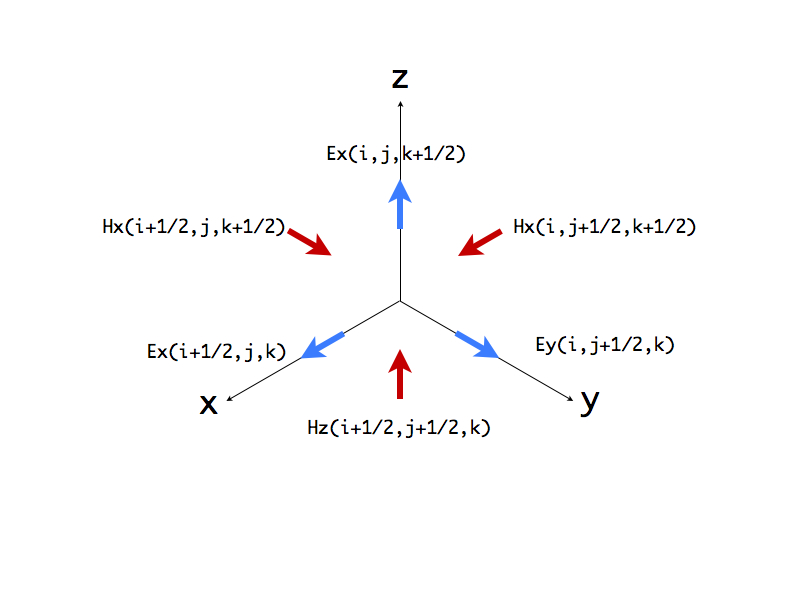
\includegraphics[scale=0.5]{images/yee-grid.jpg}\\
  Fig 2.1
\end{center}

\begin{center}
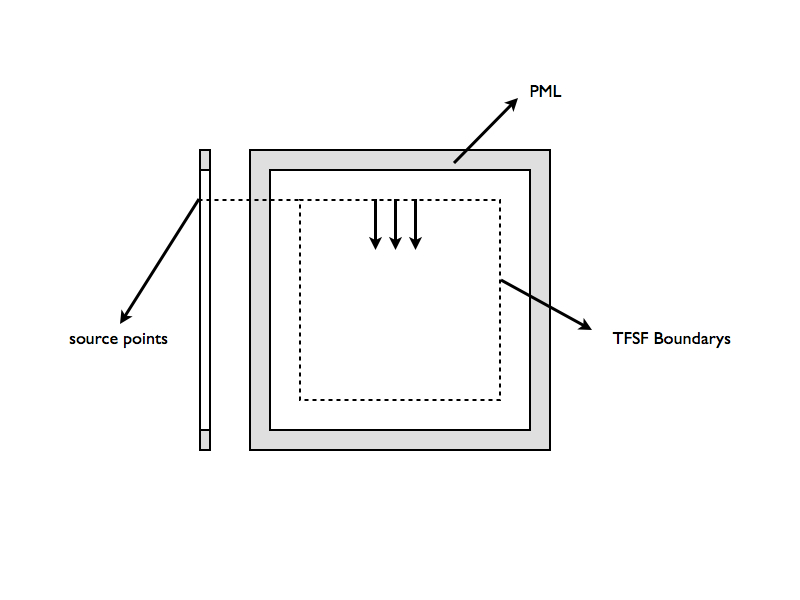
\includegraphics[scale=0.5]{images/tfsf.jpg}\\
Fig 2.2
\end{center}

\begin{center}
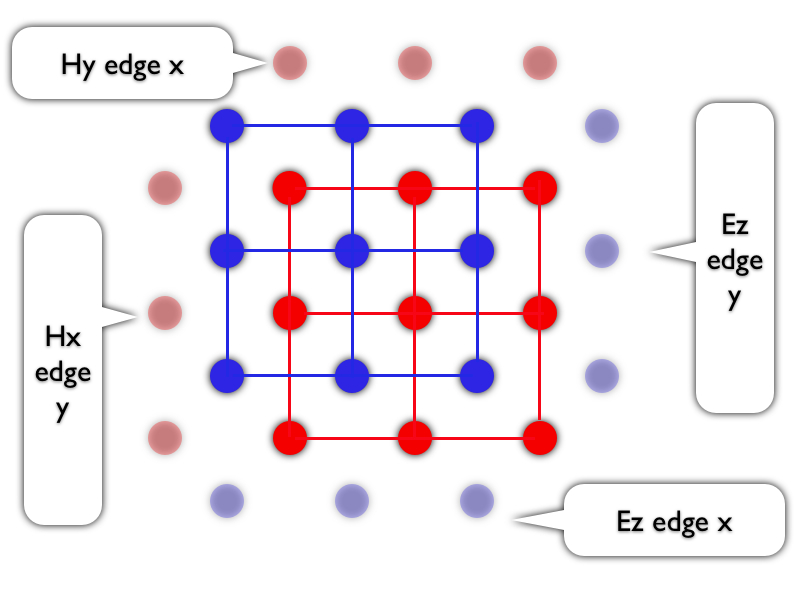
\includegraphics[scale=0.5]{images/pbc.jpg}\\
Fig 2.3
\end{center}



\chapter{The yaFDTD Framework}
\section{Yet Another FDTD Framework}

Don't reinventing the wheels. This is a famous idiom handed down from the era of industrial society. In software
engineering, there is also a common derivation of the concept: Don't Repeat Yourself (DRY). It shows understanding how
to reuse existed codes to accelerate new projects is just like earning a silver bullet for software developing. That is
why the history of software devloping is also the history of seeking better ways to reuse softwares. A function as a
resuable unit became well-known after the Structural Programming languages, such as Pascal, Ada and C, had become the
mainstream. Not a long time after that, Object-Oriented Programming (OOP) languages took over the world with Class and
Object, the more general reusable units containing functions and data structures. [Sebesta, 2007]

OOP encourages developers grouping data structures under a namespace where it's not directly accessible by the rest of
the program and bundling relative functions to form Classes. By instancing a Class, Objects are created to contain
different data but have identical data structures and behaviors. OOP promised a vision: through finding pertinent
objects and factoring them into classes at right granularity, your program would be able to address future requirements
without change too much code. [Gamma et al, 1994] Projects are also speeded up by spliting workforces for each
independent piece of a program. The set of cooperating classes making up a reusable design can form a framewok for
targeted class of software. With a framework, creating a particular application is just creating some specific
subclasses of abstract class from the framework. Actually, the road to fit the prerequisite is not flat.

The hard part about designing a framework is decomposing a system into objects due to many factor: encapsulation,
granularity, flexibility, evolution, reusability and so on [Gamma et al, 1994]. A framework designer has to gambles that
one architecture will work for all applications in the domain so that a framework should be as flexible and extensible
as possible. Loose coupling is another imperative issue for preventing major repercussion in applications when doing a
minor change to the framework. Facing challenges one after another, few researchers of FDTD are willing to spend time on
proposing a design of FDTD framework of which they can take advantage.

Fortunately, Components of FDTD simulator has given us a native prototype of architecture. Every component can be just
defined as a class. The emergent problem is they have some functionalities overlapping for simple or complex situation
respectively. How to design a extensible way making complex component can be adopted when needed become the main
delimma. This chapter is aimed at proposing a experimental framework of FDTD with a special Design Pattern: Once
Decorator, making the framework can be extended with arbitrary compoments for complex situations. Whole project named
Yet Another FDTD (yaFDTD) framework was released under GPL v2 license and hosted at
\texttt{\url{http://github.com/shelling/yafdtd}}. Even it's a implementation in Python programming language, the
concepts about the split of data structures and classes can be transplanted into other languages easily.

\section{Once Decoractor}
The Decoractor Pattern is a well-known Design Pattern listed in the bestseller of Gang of Four, \textit{Design Patterns:
  Elements of Reusable Object-Oriented Software}. The book describes that the purpose of the Decorator Pattern is
attaching additional responsibilities to an object dynamically. The role of Decorators in ths pattern provide a flexible
alternative to subclassing for extending functinoality.

Similar name implies similar behavior. The Once Decorator is the mixing of Singleton Pattern and Dynamic Inheritance,
which is acting like Decorator but actually not. The most remarkable difference is the Decorator Pattern delegates all
method calls to what it decorates, i.e. all subclasses should provide the same interfaces as main component when the
Once Decorator inherits the main component dynamically to retrieve the interfaces from what it decorates when
initializing. Dynamic Inheritance also allows subclasses overwriting interfaces to adapt more complex situations as well
as attaching additional interfaces without providiong in every related class. These are advantages of the Once Decorator
Pattern.

Dynamic Inheritance induces another problem: once two instances perform inheritance, the latter would changes the
behaviors of the former. Because a FDTD simulaion needs only one main component, Singleton Pattern acts inside of the
Once Decorator for preventing modification of inheritance on identical subclass. Moreover, all subclasses save the
singleton instance in main component to ensure one and only one singleton instance can be allowed to join the
calculation.

The architecture of Once Decorator is also similar to Decorator as shown in Fig 3.1. The magic is hidden in constructor
of Decorator. Assuming main component of two dimension is named as Plane, the Decorator can be implemented as following.
\begin{code}
  class PlaneDecorator(Plane):
    def __new__(clz):
        if not clz.singleton:
            clz.singleton = object.__new__(clz)
            Plane.singleton = singleton
        return clz.singleton

    def __init__(self, orig):
        self.__dict__ = orig.__dict__
        if orig.__class__ != Plane:
            self.__class__.__bases__ = (orig.__class__,)
        return None
\end{code}
The concrete decorator subclasses would inherit the abstract decorator class and invoke the constructor when
initializing. The constructor does two things: exporting all instance variables to a new instance created from any
concrete decorator and making the concrete decorator inheriting the another concrete decorator from the original
instance.

The two actions save the instance variables and make later decorators can overwrite interfaces of prior decorators
through inheritance in concise relation.

\section{Freespace Component}
The freespace component serve as main component in the architecture of Once Decorator. It stores fields components as
instance variables and provides the interfaces to update fields by the rules of freespace. The fields components are
utilized by concrete decorators which have to inherit main component. And about interfaces, there is a big trick
here. Comparing the Eq.\ref{eq:pmldx} and Eq.\ref{eq:dx3d}, the curl part are are not changed. Apparently it necessary
to provide interfaces for these reusable part. The $curl\_ex$ and $curl\_hx$ is a example here.
\begin{code}
    def curl_ex(self):
        res = numpy.zeros(self.shape)
        (x,y,z) = self.shape
        for i in range(x):
            for j in range(y-1):
                for k in range(z-1):
                    res[i,j,k] = self.ezfield[i,j+1,k] - self.ezfield[i,j,k] 
                               - self.eyfield[i,j,k+1] + self.eyfield[i,j,k]
        return res

    def curl_hx(self):
        res = numpy.zeros(self.shape)
        (x,y,z) = self.shape
        for i in range(x):
            for j in range(y):
                for k in range(z):
                    res[i,j,k] = self.hzfield[i,j,k] - self.hzfield[i,j-1,k] 
                               - self.hyfield[i,j,k] + self.hyfield[i,j,k-1]
        return res
\end{code}
The return value is a 2D array saving the value of curl for each point. with the interface, Eq.\ref{eq:dx3d} and
Eq.\ref{eq:bx3d} appear a elegant view in source code.
\begin{code}
    def update_dfield(self):
        self.dxfield += 0.5 * self.curl_hx()
        self.dyfield += 0.5 * self.curl_hy()
        self.dzfield += 0.5 * self.curl_hz()
        return self
    def update_bfield(self):
        self.bxfield -= 0.5 * self.curl_ex()
        self.byfield -= 0.5 * self.curl_ey()
        self.bzfield -= 0.5 * self.curl_ez()
        return self
\end{code}
And the E field and H field are just copied from D and B in freespace. Handlers for material are left to implment in
Dispersion concrete decorator. 
\begin{code}
    def update_efield(self):
        self.exfield = self.dxfield.copy()
        self.eyfield = self.dyfield.copy()
        self.ezfield = self.dzfield.copy()
        return self

    def update_hfield(self):
        self.hxfield = self.bxfield.copy()
        self.hyfield = self.byfield.copy()
        self.hzfield = self.bzfield.copy()
        return self
\end{code}



\section{PBC Component}
To make PBC component work, surrounded edges must be appended as instance variables and participate the calculation of
curl part. For minimizing trivial code, this can be implenented in Freespace component. For example, the $curl\_ex$ in
2D may invole edges as following.
\begin{code}
    def curl_ex(self):
        res = numpy.zeros(self.shape)
        (x,y) = self.shape
        for i in range(x):
            for j in range(y-1):
                res[i,j] = self.ezfield[i,j+1] - self.ezfield[i,j]
        for i in range(x):
            res[i,y-1] = self.ezedgey[i] - self.ezfield[i,y-1]  # invole edges
        return res
\end{code}
The duty of PBC component now remain locating the the PBC and update the edge components. Instance variables
\texttt{pbcx} and \texttt{pbcy} are used to verify which edges should serve.
\begin{code}
    def pbc(self, x=True, y=True):
        self.pbcx = x
        self.pbcy = y
        return self

    def update_epbc(self):
        if self.pbcx:
            self.ezedgex = self.ezfield[0,:] # pbc x, TM
            self.eyedgex = self.eyfield[0,:] # pbc x, TE
        if self.pbcy:
            self.ezedgey = self.ezfield[:,0] # pbc y, TM
            self.exedgey = self.exfield[:,0] # pbc y, TE
        return self

    def update_hpbc(self):
        xmax = self.shape[0]-1
        ymax = self.shape[1]-1
        if self.pbcx:
            self.hyedgex = self.hyfield[xmax,:] # pbc x, TM
            self.hzedgex = self.hzfield[xmax,:] # pbc x, TE
        if self.pbcy:
            self.hxedgey = self.hxfield[:,ymax] # pbc y, TM
            self.hzedgey = self.hzfield[:,ymax] # pbc y, TE
        return self
\end{code}


\section{UPML Component}
The hard part of UPML implementation is the summation term. The solution is deploying auxiliary variables to sum current
values of curl and participate updating. In the case of 2D, (\ref{eq:pmldx}), (\ref{eq:pmldy}), and (\ref{eq:pmldz})
was implemented as following.
\begin{code}
    def update_dfield(self):
        self.idx += self.curl_hx()
        self.idy += self.curl_hy()
        self.dxfield = self.j3 * self.dxfield 
                     + self.j2 * 0.5 * ( self.curl_hx() + self.i1 * self.idx )
        self.dyfield = self.i3 * self.dyfield 
                     + self.i2 * 0.5 * ( self.curl_hy() + self.j1 * self.idy )
        self.dzfield = self.i3 * self.j3 * self.dzfield 
                     + self.i2 * self.j2 * 0.5 * self.curl_hz()
        return self
\end{code}
The summation of $curl\_hx$ and $curl\_hy$ are saved in \texttt{idx} and \texttt{idy}. The variables defined in
(\ref{eq:v3}), (\ref{eq:v2}), (\ref{eq:v1}) are saved as arrays \texttt{i1}, \texttt{i2}, \texttt{i3}, \texttt{j1},
\texttt{j2}, \texttt{j3} which are mapping coefficients to every point in computational domain. In Sullivan's example,
he used one dimension arrays to save memory. However, it's more intuitive and programmable using array having
dimension(s) the same as field variables.

The multiplication operator of numpy ndarray do multiplication for each pair having the same index like inner
product. That makes the code clean as in mathematics. In any programming language allowing operator overloading,
including Perl, Ruby, C++ and Java, it is a better alternative using a function as middleware to enclose for loops
rather than writing for loop here directly.

\section{TF/SF Component}
Concepts of TF/SF Component are easy to grasp. However, the theory left a big blank canvas for implementation because
there are eight types in two dimension and twelve types in three dimension. A intuitive implementation is categorizing
by incident direction to be XTFSF, YTFSF, and ZTFSF (only in 3D). An XTFSF can be TM or TE mode and each mode can be
rectangle layout or infinite layout working with PBC (Fig 3.2), YTFSF and ZTFSF too. By example of YTFSF in two
dimension, the constructor appends two auxiliary 1D source as well as masks boundary of TFSF in two direction. 
\begin{code}
    def __init__(self, orig):
        super(YTFSFPlane, self).__init__(orig)
        self.tminc = String(self.shape[1])
        self.teinc = String(self.shape[1])
        self.xtfsf = [10, self.shape[0]-10]
        self.ytfsf = [10, self.shape[1]-10]
        return None
\end{code}
The rest is two more interfaces to insert D and B at TFSF boundary. To simplify, TE and TM mode are inserted at the same
time. If only one mode is needed, no updating on the unnecessary auxiliary 1D source in main script could disable
it. This design leads to more overhead but creates elegant depiction. The next big trick is to examinate whether the
boundaries in x direction are \texttt{[None, None]}. If the assertion is true, regard TFSF itself as a layout infinite
at x direction. Otherwise, it's a rectangle layout should update boundaries in x direction.
\begin{code}
    def update_dtfsf(self):
        if self.xtfsf == [None, None]:
            self.dzfield[:, self.ytfsf[0]]
            += 0.5 * self.tminc.hfield[self.ytfsf[0]-1]
            self.dzfield[:, self.ytfsf[1]] 
            -= 0.5 * self.tminc.hfield[self.ytfsf[1]]
            self.dxfield[:, self.ytfsf[0]]  
            -= 0.5 * self.teinc.hfield[self.ytfsf[0]-1]
            self.dxfield[:, self.ytfsf[1]]  
            += 0.5 * self.teinc.hfield[self.ytfsf[1]]
        else:
            # y edge
            self.dzfield[self.xtfsf[0]:self.xtfsf[1]+1, self.ytfsf[0]]  
            += 0.5 * self.tminc.hfield[self.ytfsf[0]-1]
            self.dzfield[self.xtfsf[0]:self.xtfsf[1]+1, self.ytfsf[1]]  
            -= 0.5 * self.tminc.hfield[self.ytfsf[1]]
            self.dxfield[self.xtfsf[0]:self.xtfsf[1]+1, self.ytfsf[0]]  
            -= 0.5 * self.teinc.hfield[self.ytfsf[0]-1]
            self.dxfield[self.xtfsf[0]:self.xtfsf[1]+1, self.ytfsf[1]]  
            += 0.5 * self.teinc.hfield[self.ytfsf[1]]

            # x edge
            self.dyfield[self.xtfsf[0],   self.ytfsf[0]:self.ytfsf[1]+1] 
            += 0.5 * self.teinc.hfield[self.ytfsf[0]:self.ytfsf[1]+1]
            self.dyfield[self.xtfsf[1]+1, self.ytfsf[0]:self.ytfsf[1]+1] 
            -= 0.5 * self.teinc.hfield[self.ytfsf[0]:self.ytfsf[1]+1]
        return self


    def update_btfsf(self):
        if self.xtfsf == [None, None]:
            # y edge
            self.bxfield[:, self.ytfsf[0]-1]
            += 0.5 * self.tminc.efield[self.ytfsf[0]]
            self.bxfield[:, self.ytfsf[1]]  
            -= 0.5 * self.tminc.efield[self.ytfsf[1]]
            self.bzfield[:, self.ytfsf[0]-1]
            += 0.5 * self.teinc.efield[self.ytfsf[0]]
            self.bzfield[:, self.ytfsf[1]]  
            -= 0.5 * self.teinc.efield[self.ytfsf[1]]
        else:
            # y edge
            self.bxfield[self.xtfsf[0]:self.xtfsf[1]+1, self.ytfsf[0]-1] 
            += 0.5 * self.tminc.efield[self.ytfsf[0]]
            self.bxfield[self.xtfsf[0]:self.xtfsf[1]+1, self.ytfsf[1]]   
            -= 0.5 * self.tminc.efield[self.ytfsf[1]]
            self.bzfield[self.xtfsf[0]:self.xtfsf[1]+1, self.ytfsf[0]-1] 
            += 0.5 * self.teinc.efield[self.ytfsf[0]]
            self.bzfield[self.xtfsf[0]:self.xtfsf[1]+1, self.ytfsf[1]]   
            -= 0.5 * self.teinc.efield[self.ytfsf[1]]

            # x edge
            self.byfield[self.xtfsf[0]-1, self.ytfsf[0]:self.ytfsf[1]+1] 
            -= 0.5 * self.tminc.efield[self.ytfsf[0]:self.ytfsf[1]+1]
            self.byfield[self.xtfsf[1],   self.ytfsf[0]:self.ytfsf[1]+1]
            += 0.5 * self.tminc.efield[self.ytfsf[0]:self.ytfsf[1]+1]
        return self
\end{code}

\section{Dispersion Component}
Owing to the demand of supports to multiple poles in Eq.\ref{eq:dispersive}, the dispersion component has to be splited
into two part. The $\epsilon_r$ are saved in main decorated component to participate calculation after retrieving the
summation of $J_p$. Oppositely, $J_p$ saving $a,b,c,d$ coefficients is implemented as a independent class not involving
in Once Decorator inheritance structure.

One more decorator is needed to append $\epsilon_r$ to main component and overwrite the \texttt{update\_efield} method
as following. 
\begin{code}
    def update_efield(self, *polar):
        self.exfield  = self.dxfield.copy()
        self.eyfield  = self.dyfield.copy()
        self.ezfield  = self.dzfield.copy()
        for p in polar:
            self.exfield -= p.x
            self.eyfield -= p.y
            self.ezfield -= p.z
        self.exfield /= self.epsilon_rx
        self.eyfield /= self.epsilon_ry
        self.ezfield /= self.epsilon_rz
        return self
\end{code}
The variable \texttt{*polar} with star declares it can receive arbitrary arguments and act as an array. In the middle
for loop, $E$ field uses the values copied from $D$ field to subtract the $J_p$. Then $\epsilon_r$ divides $E - \sum
J_p$ in latter three lines. The reason each E field component has its own appointment of $\epsilon_{r}$ has been
explained in Section \ref{sec:modeling}.

The second part of dispersion component is $J_p$. The constructor of $J_p$ does two things. The first is calculating
$C1$, $C2$, and $C3$ from $a,b,c,d$ coefficients. The other is appending instance variables for saving polarized
displacement of recent three steps. From Eq.\ref{eq:polarized_displacement}, the method \texttt{update} was implemented
as following. The strategy to distinguish material is slightly different from modeling $\epsilon_r$. Logically, one pole
saves one set of coefficients, so that it's not necessary saving coefficients as arrays. Masks are a better design here.
\begin{code}
    def update(self, plane):
        self.xp2 = self.xp
        self.yp2 = self.yp
        self.zp2 = self.zp
        self.xp = self.x
        self.yp = self.y
        self.zp = self.z
        self.x = self.c1*self.xp + self.c2*self.xp2 + self.c3*plane.exfield*self.maskx
        self.y = self.c1*self.yp + self.c2*self.yp2 + self.c3*plane.eyfield*self.masky
        self.z = self.c1*self.zp + self.c2*self.zp2 + self.c3*plane.ezfield*self.maskz
        return self
\end{code}
In the main FDTD loop, the two parts constructed above collaborate after retrieving current $D$ field. All poles update
themselves with previous $E$ field and $E$ field finds its current values from all poles.
\begin{code}
  plane.update_dfield()

  # three poles are defined 
  drude_pole.update(plane)
  lorentz_pole1.update(plane)
  lorentz_pole2.update(plane)

  plane.update_efield(drude_pole, lorentz_pole1, lorentz_pole2) # allow arbitrary poles 
\end{code}

\section{MPI Edge Component}
Because there is no possibility to overcome the time complexity $\Omicron (3)$ in 3D and $\Omicron (2)$ in 2D For
investigating some huge structure, parallelization is a imperative support in FDTD. Recently famous Tactics to
parallelization include Cuda, Pthreads API, OpenMP API, and MPI standard. For well integrating with numpy used in
yaFDTD, mpi4py, the brother package implementing MPI Standard, was pick out here. 

In the slant of MPI, computational domain of FDTD can be splited into many fragments on different memory block and
manipulated by different CPU. Because data fragments are independent with others, at edges of computational domain, it
needs to exchange data. APIs of MPI serve here.

Invoking APIs of MPI in main script is a quick and dirty solution in vary examples and tutorials. It's possible wrapping
MPI actions in a class as a Decorator in our architecture. 
\begin{code}
  
\end{code}


\clearpage
\begin{center}
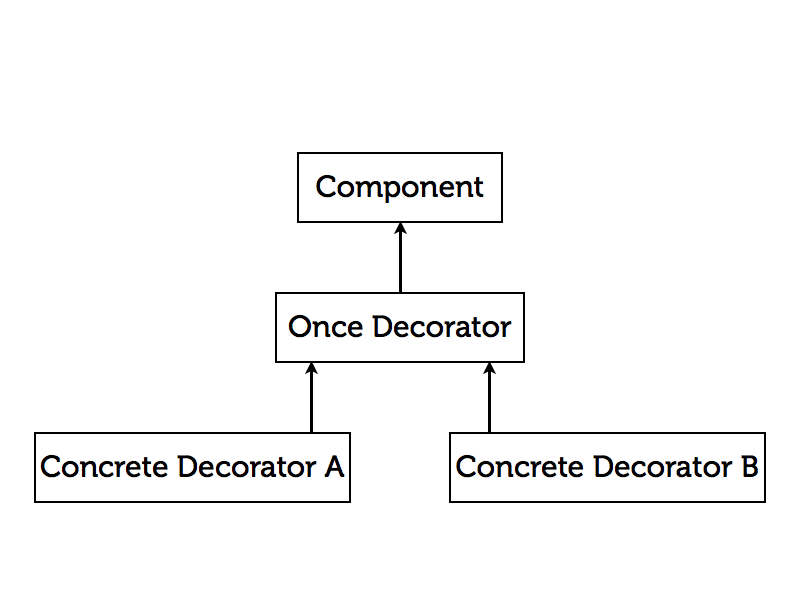
\includegraphics[scale=0.5]{images/once-decorator.jpg}\\
Fig 3.1
\end{center}
\begin{center}
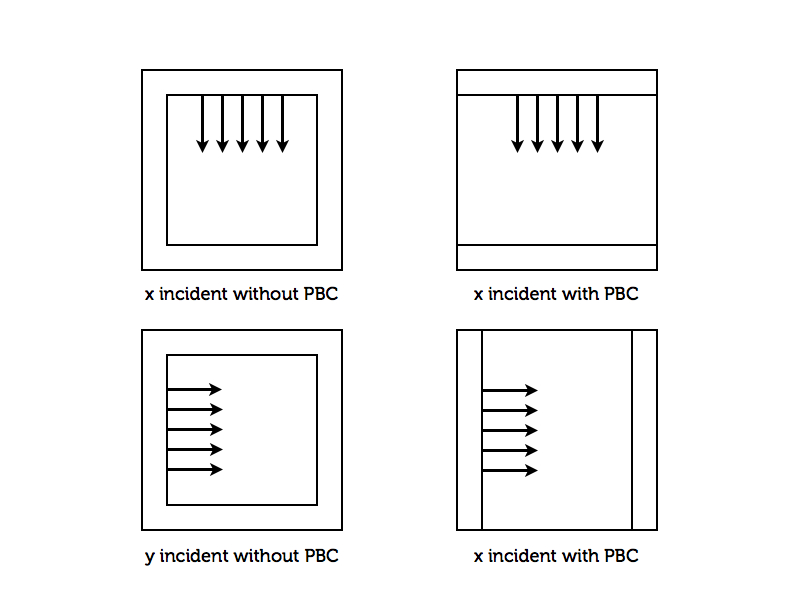
\includegraphics[scale=0.5]{images/tfsf-pbc.jpg}\\
Fig 3.2
\end{center}



\chapter{Applications about Surface Plasmon Structures}
\section{examination}
The surface plasmonic structures become popular in this two decades owing to plasmonic waveguides admit optical waves
transmitting in subwavelength structures having metal-dielectric interfaces specially in nano-scale. The conduction
electrons oscillate in the longitudinal direction and the Maxwell's equations show the solution is electromagnetic
fields confined near the interface of metal.

Single silver rod may one of the most simple metal-dielectric interface. Phasor distribution of single silver rod is
easy to obtain via frequency domain method such as Multiple-Scattering method. By performing Fourier transform on
timeline of FDTD result reaching steady state, a good approximation is expected. To ensure the yaFDTD framework to carry
out a credible result, comparison result between exact solution and FDTD is a good index.

The example here is a nano cylinder with radius 25 nm. The cylinder material is silver simulated using Drude Model
with following parameters: $\epsilon_r = 8.926$, $\omega_p = 9.39 \times 10^{15}$ rad/s, and $\gamma_p = 3.14 \times
10^{13}$ rad/s.  There would be one more thing remarkable before starting simulation to acquire better result. Although
the UPML has excellent performance for absorbing propagatin waves; however, the evanescent waves still grows field
intensity up inside the UPML. To prevent the reflection from PML interact with the scatters. It need extra space between
PML and scatters. Here we set the grid size to be 1 nm and make whole space being 500 nm $\times$ 500 nm.

Final arrangement is shown in Fig 4.1. Plane wave in $\mathrm{TE_z}$ mode is impinged in x-direction with wavelength
347.5 nm. Fig 4.2 shows the Re\{$H_z$\} profiles of phasor distribution when reaching steady state after 100 periods of
plane wave. Fig 4.3 shows the exact solution of Re\{$H_z$\} profiles. and numerical error shown in Fig 4.4 is calculated
by subtracting the result from FDTD with the result from exact solution. The inaccuracy is small than 0.1 with the
simplest Stair-Case scheme. In general, it good enough to apply the framework on more complex cases.

\section{Silver Rods Open Cavity}
Using nano-scale structure to design devices for confining or guiding light may be the major challenges in optical
researches. When the surface plasmon resonance provides dramatic local-field enhancement, a series of silver rods can
has the ability to guide light in finite length through near-field coupling. In additions, Confinement of light can be
also obseved by arrange silver rods to enclose space [Ng, 2006]. Local-field enhancement plays other important role like
gain media in laser that mean the enclosed space can form an open cavity. Here we study the phasor characteristics of a
silver rods open cavity proposed recently.

The open cavity forms of three silver nanocylinder pairs. Fig 4.5 shows the geometry configuration of three pairs of
silver nanocylinders. The interparticle distance is $d$. The interpair distance is $d_p$. The radius of nanocylinders is
$r$. The three pair structures are illuminated with a plane wave of $\mathrm{TE_z}$ polarized mode. Drude Model is used
again in this simulation but parameters is set using the experimental data from Palik. Computational region is set to be
500 nm $\times$ 500 nm and 20 nm UPML is surrounded outside whole region.

Due to the fact the optical response of nanoparticles would act as dipoles when the size of nanoparticles are far
smaller than wavelength of impinged plane wave. The interaction between nanoparticles is similar to the interaction
between dipoles. The higher multipole behavior becomes apparent with increasing size of nanoparticles. For the reason,
the radius of nanocylinders should change the near-field optical response of the open cavity.

Previous study shows the maximum intensity in chamber occrurs when the ratio of wavelength and nanocylinder radius is
around 11 and 12. Two remarkable cases are also shown in phasor distribution. The first case impinges plane wave in
wavelength 460 nm and the six nanocylinders are set as $r = 36$ nm, $d = d_p = 20$ nm, which the ratio is $\lambda /r
= 12.7$. The second case impinges plane wave in wavelength 650 nm and nanocylinders are set as $r = 58$ nm, $d = d_p =
20$ nm, which the ratio is $\lambda /r = 11.2$ . For futher testing of performance of the yaFDTD framework we directly
perform this two cases again because the numerical simulation error usually arises as the field intensity is enhanced
severely.

Fig 4.6 and 4.11 shows the steady state total E field phasor distribution for the first and second case mentioned above
respectively. Comparing with the result shown in previous study (Fig 4.7 and Fig 4.12), the phasor distribution of
yaFDTD can fit it good. 

Fig 4.8 and 4.9 also shown the the partial E field phasor distribution for $\mathrm{E_x}$ and $\mathrm{E_y}$ in the
first case. Fig 4.13 and Fig 4.14 are for the second case. It can be observed the $\mathrm{E_x}$ component is dominant
in the gaps between pairs and the $\mathrm{E_y}$ component is dominant inside the gaps of each pairs. This shows that we
can partially manipulate the $\mathrm{E_x}$ and $\mathrm{E_y}$ by change the distance in pairs $d$ and distance between
pairs $d_p$ to reduce the interaction of dipoles.  For example, when we change the $d_p$ to be 40 nm in the first case
(Fig 4.15), the $\mathrm{E_x}$ would almost disappear (Fig 4.18 and Fig 4.19). The |$\mathrm{E}$| of yaFDTD and previous
study are also shown in Fig 4.16 and Fig 4.17.

\clearpage
\begin{center}
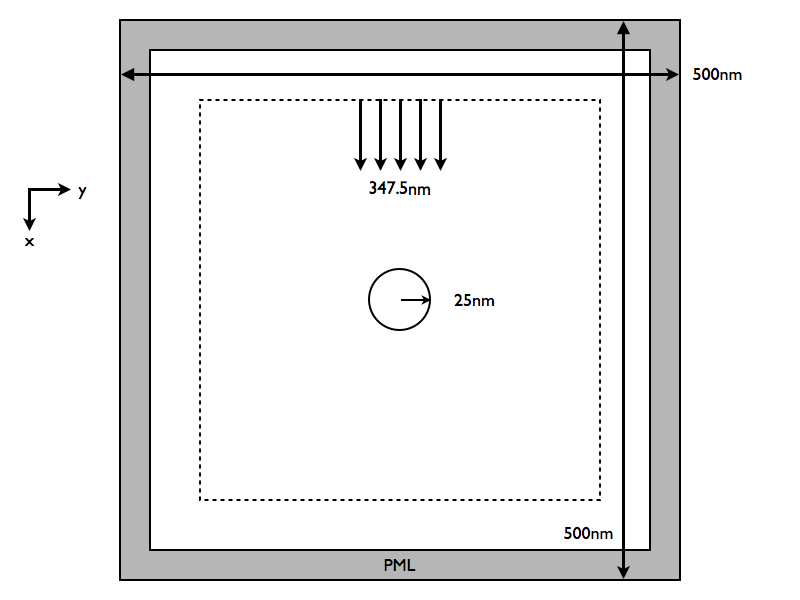
\includegraphics[scale=0.5]{images/single-rod-config.jpg}\\
Fig 4.1
configuration of single silver rods
\end{center}
\begin{center}
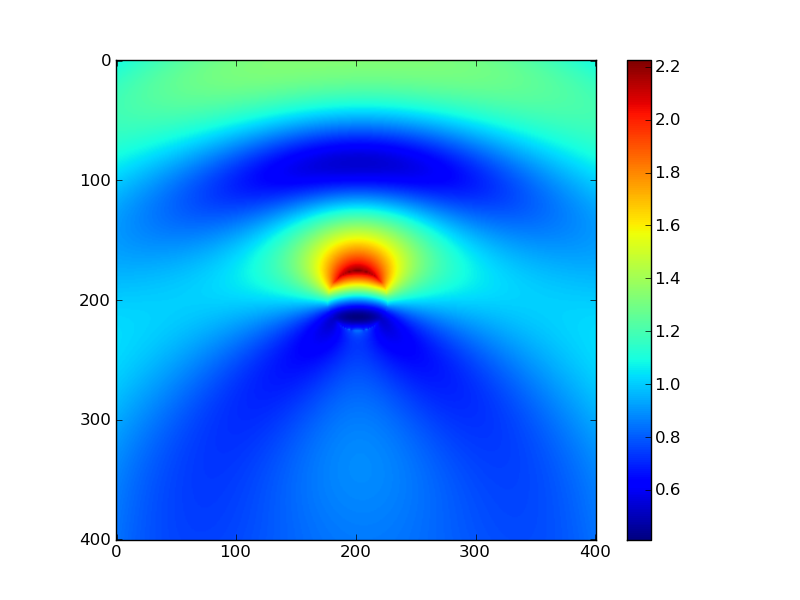
\includegraphics[scale=0.8]{images/phasor-exam-fdtd.png}\\
Fig 4.2
phasor distribution of $mathrm{H_z}$, calculated by yaFDTD
\end{center}
\begin{center}
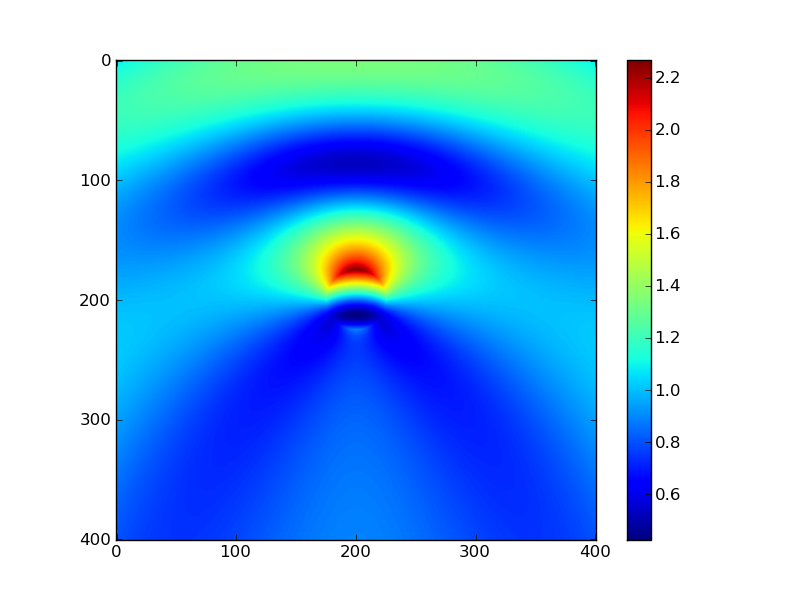
\includegraphics[scale=0.8]{images/phasor-exam-exact.png}\\
Fig 4.3
phasor distribution of $mathrm{H_z}$, exact solution
\end{center}
\begin{center}
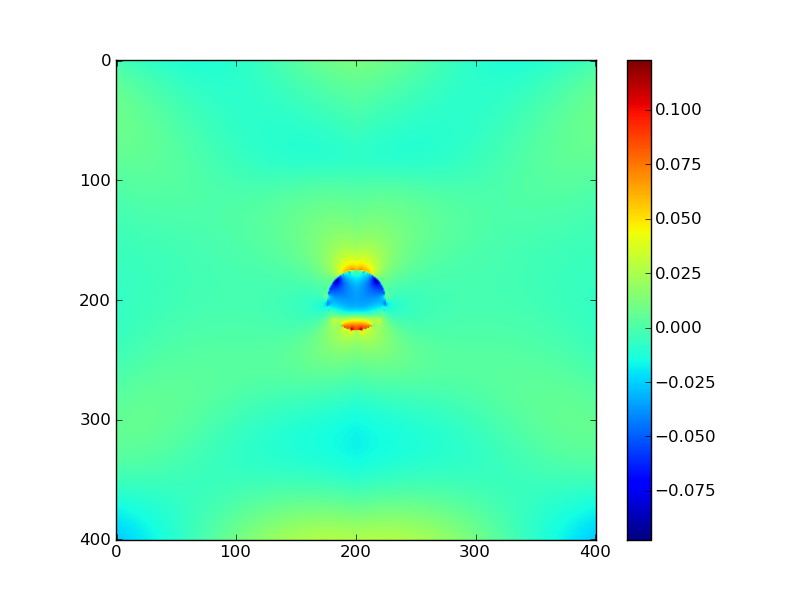
\includegraphics[scale=0.8]{images/errors.png}\\
Fig 4.4
numerical error between yaFDTD and exact solution
\end{center}
\begin{center}
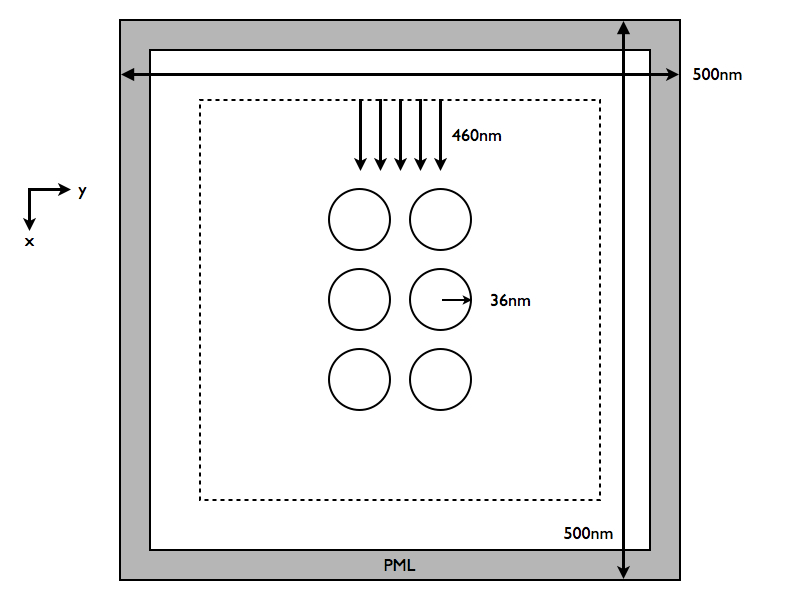
\includegraphics[scale=0.5]{images/open-cavity-config.jpg}\\
Fig 4.5
configuration of three pairs of silver nanocylinders
\end{center}
\begin{center}
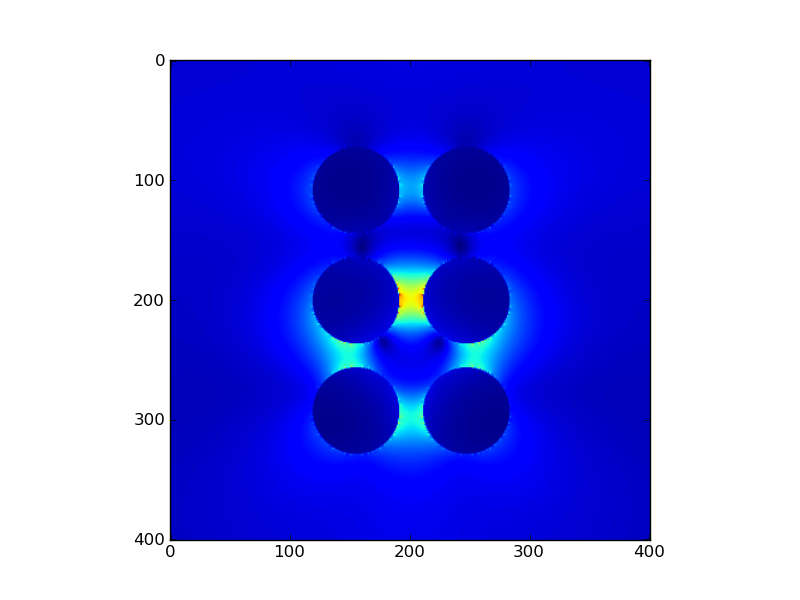
\includegraphics[scale=0.8]{images/etotal.png}\\
Fig 4.6
phasor distribution of $|E|$ for the case $\lambda = 460nm, r = 36nm, d = d_p = 20nm$, calculated by yaFDTD
\end{center}
\begin{center}
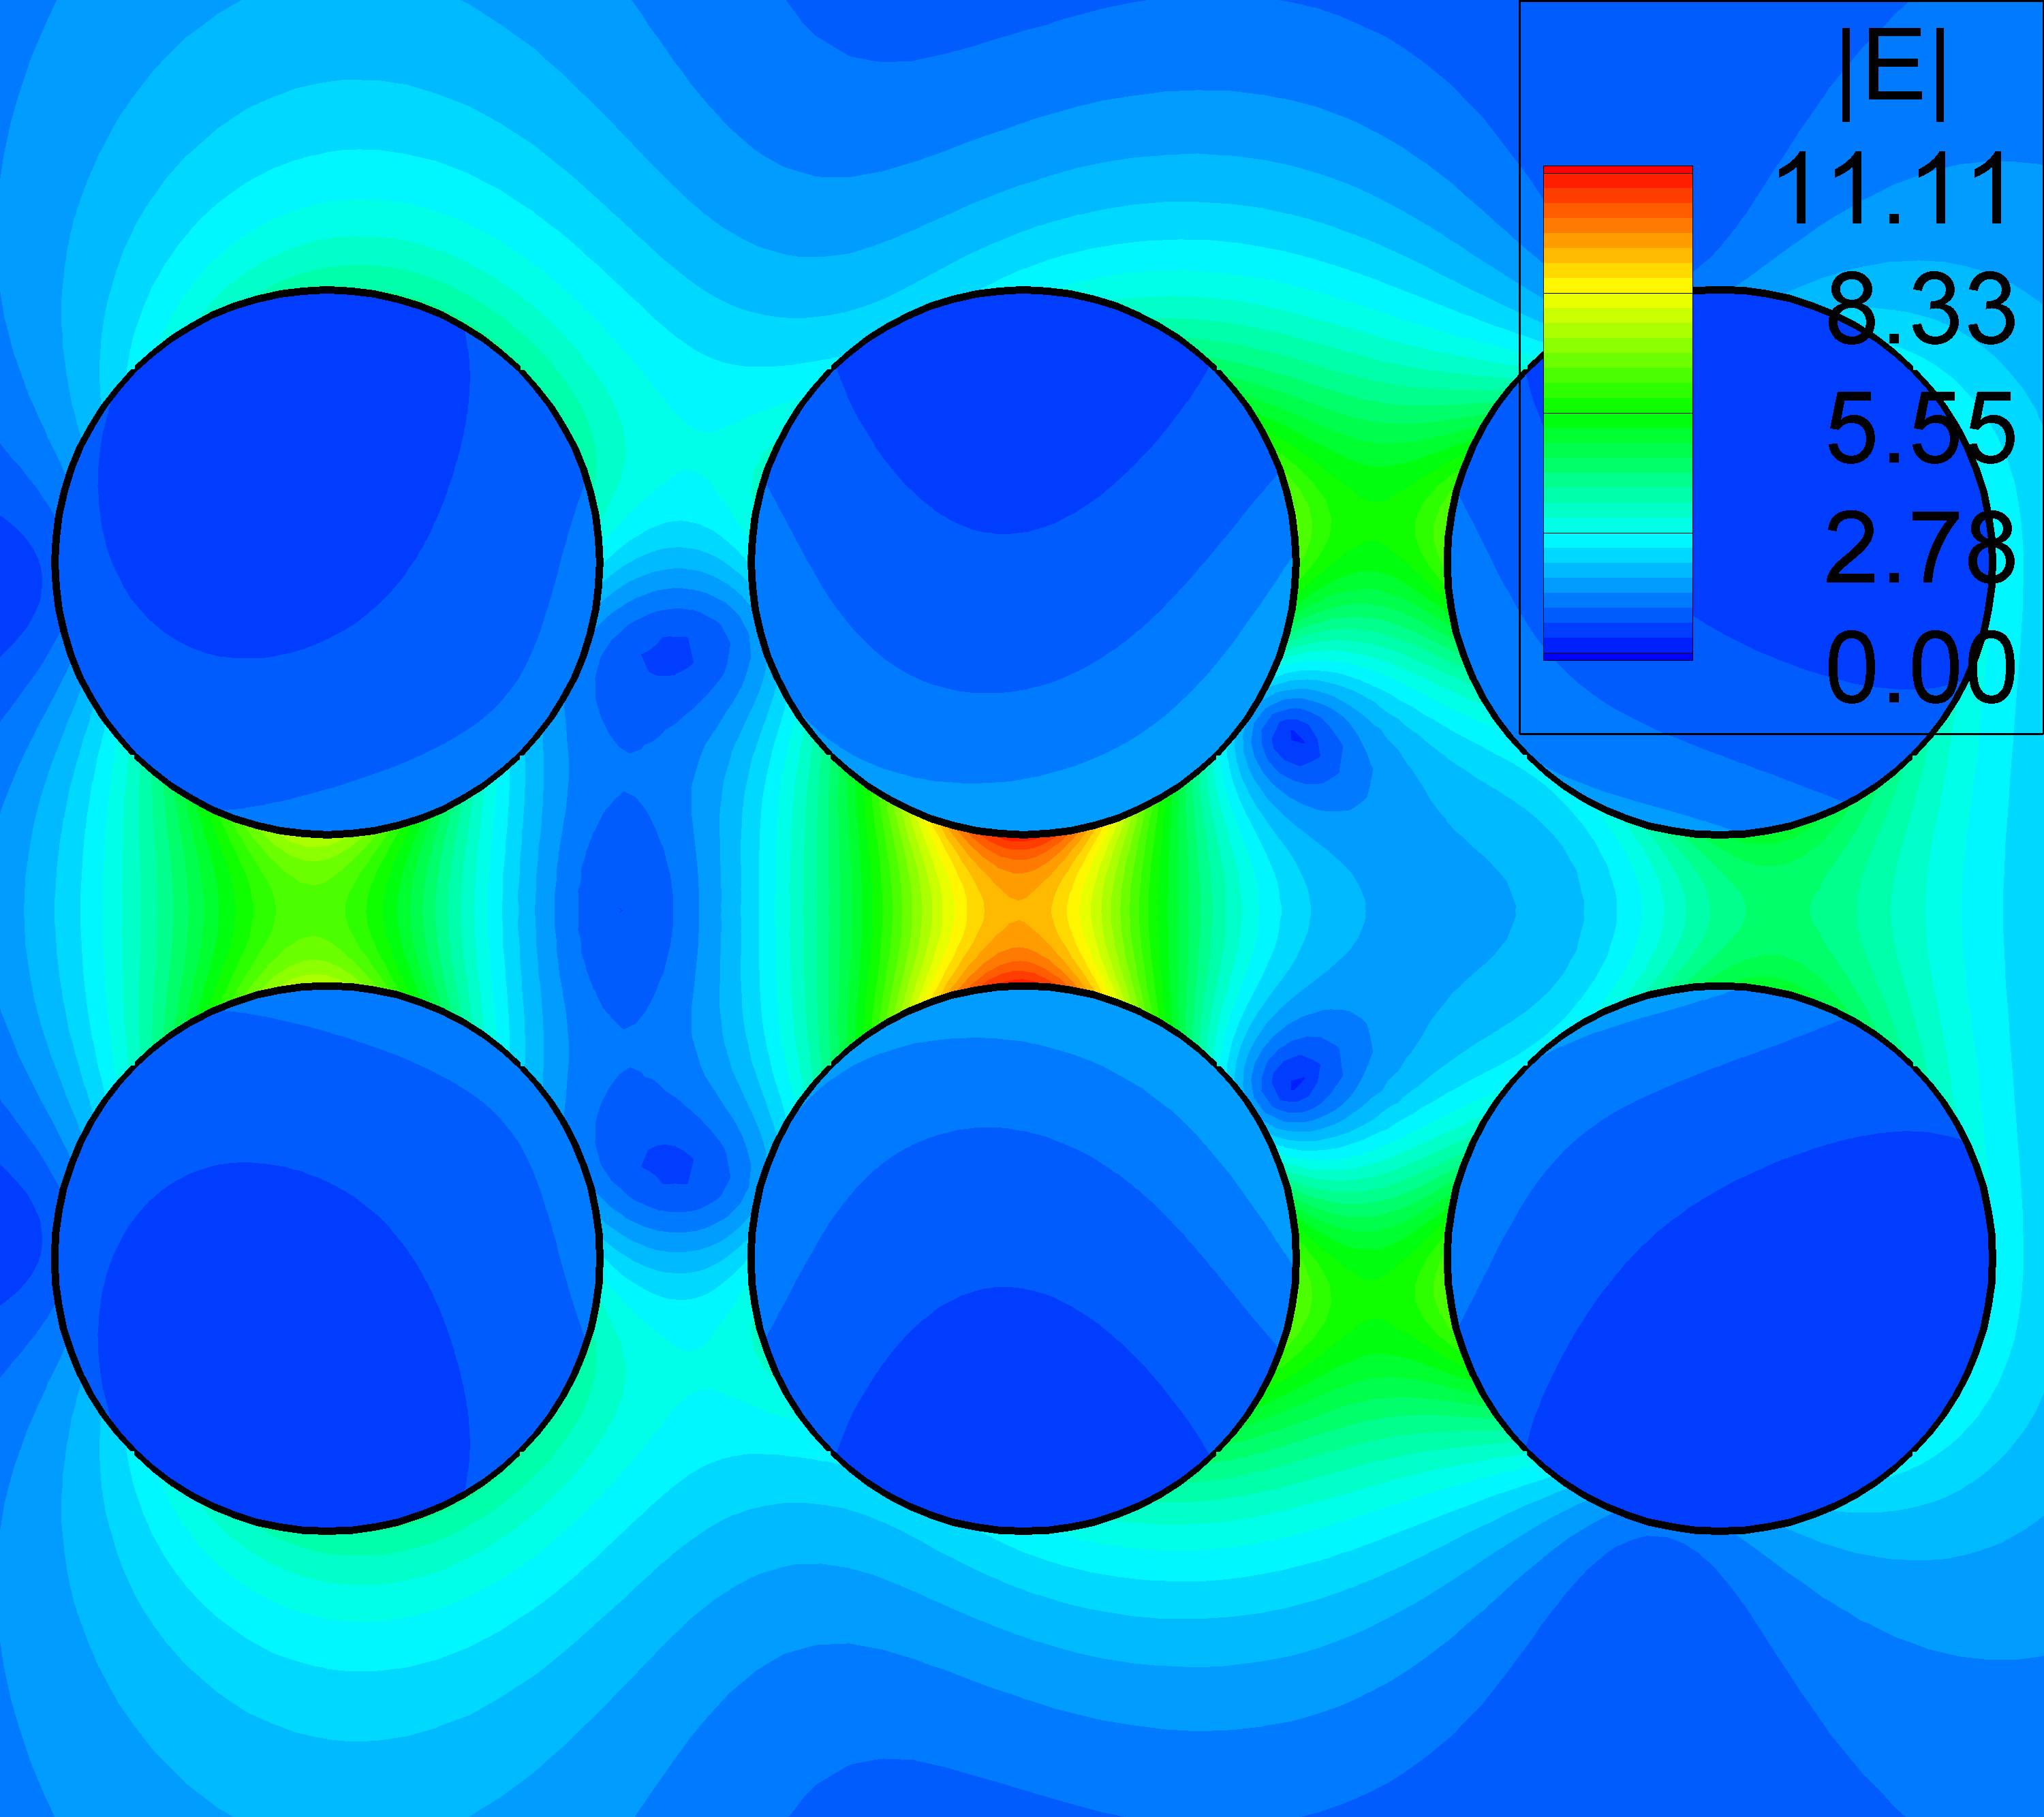
\includegraphics[scale=0.1]{images/r36.png}\\
Fig 4.8
phasor distribution of $|E|$ for the case $\lambda = 460nm, r = 36nm, d = d_p = 20nm$, in previous study
\end{center}
\begin{center}
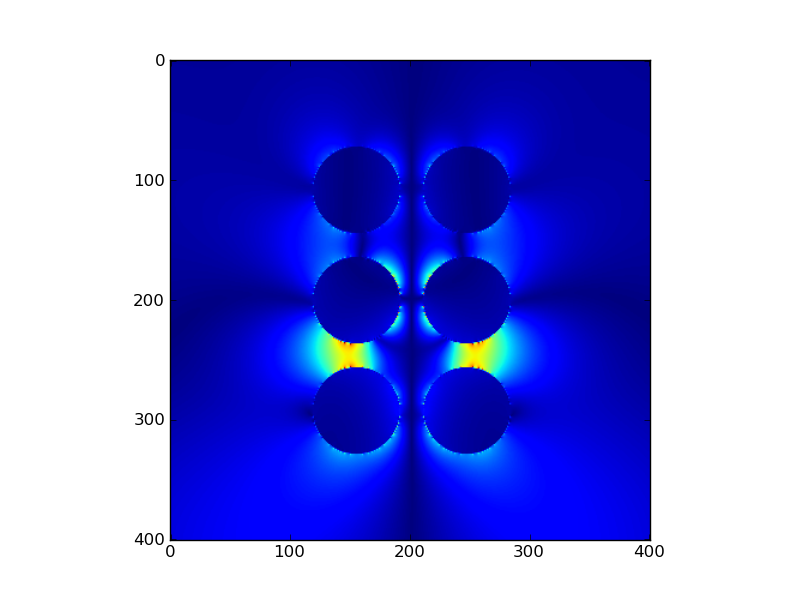
\includegraphics[scale=0.8]{images/ex.png}\\
Fig 4.9
phasor distribution of $|E_x|$ for the case $\lambda = 460nm, r = 36nm, d = d_p = 20nm$, calculated by yaFDTD
\end{center}
\begin{center}
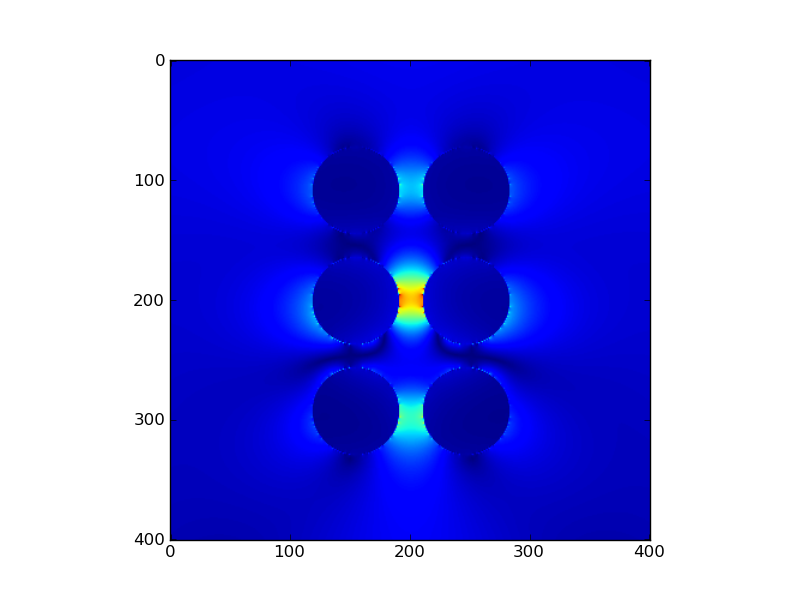
\includegraphics[scale=0.8]{images/ey.png}\\
Fig 4.10
phasor distribution of $|E_y|$ for the case $\lambda = 460nm, r = 36nm, d = d_p = 20nm$, calculated by yaFDTD
\end{center}




\chapter{Conclusion}
In this research, Maxwell's equations are reinvestigated to be a more symmetrical forms for being programmable easily
And the possibility to refactor Maxwell's equtions into a bunch of fragments is also be studied. By importing the
concepts of Structural Programming and Object-Oriented Programming, a blueprint of forming a FDTD simulator by assemble
well-prepared components appears before our eyes. It admits the newbies starting simulations without understand details
of each components. For design five common components in FDTD method: Freespace, Perfectly Matched Layers, Dispersive
Materials, Total Field / Scatter Field plane wave source, and Bloch Periodic Boundary Conditions, fragments of Maxwell's
equations are spreaded into different classes. For assembling all components well, a Design Pattern, Once Decorator, is
proposed. By the abilities of this Design Pattern, It's possible to append or exchange new components into future
simulation without considerable changes in other components have been written. Existed five components is also gathered
as a tiny framework.

The structures formed of silver nanocylinders are also studied. In single silver rods case, the phasor distribution
calculated by FDTD is compared with exact solution. This case shows that the accuracy of the tiny framework is
credible. An open cavity forms of three silver nanocylinders pairs are also studied. Phasor calculation shows the open
cavity has the maximum resonance when the ratio of wevelength of impinging plane wave and the radius of nanocylinders is
around 11 and 12. Partially phasor distribution of $|\mathrm{E_x}|$ and $|\mathrm{E_y}|$ also shows the details of
dipole interaction. It implies increasing distance between pairs $|\mathrm{E_y}|$ would be weaken and $|\mathrm{E_x}|$
has the same change when distance inside each pairs increase due to less coupling of near-field.




%% \appendix
%% \chapter{Comparing ADE, RC and ZT}
%% \paragraph{{\msjh Debye Model - RC}}
\begin{displaymath}
  \epsilon_r^*(\omega) = \epsilon_r + \frac{\sigma}{j\omega \epsilon_0} + \frac{\Delta \epsilon_p}{1+j\omega \tau_p}
\end{displaymath}
\begin{displaymath}
  \begin{split}
    \widetilde{D}(\omega) & = \epsilon_r^*(\omega)\widetilde{E}(\omega)\\
    & = \epsilon_r\widetilde{E}(\omega) + \frac{\sigma}{j\omega\epsilon_0}\widetilde{E}(\omega) + \frac{\Delta \epsilon_p}{1+j\omega \tau_p}\widetilde{E}(\omega)
  \end{split}
\end{displaymath}
\begin{displaymath}
  \widetilde{D}(t) = \epsilon_r\widetilde{E}(t) + \frac{\sigma}{\epsilon_0}\int_0^t\widetilde{E}(t')dt' + \int_0^t\frac{\Delta \epsilon_p}{\tau_p}e^{-\frac{t'-t}{\tau_p}}\widetilde{E}(t')dt'
\end{displaymath}
\begin{equation}
  \widetilde{D}^n = \epsilon_r\widetilde{E}^n + \frac{\sigma}{\epsilon_0}\Delta t\sum_{i=0}^{n}\widetilde{E}^i + \frac{\Delta \epsilon_p}{\tau_p}\Delta t \sum_{i=0}^{n} e^{-\frac{n-i}{\tau_p}\Delta t}\widetilde{E}^i
\end{equation}
The second term, dissipated displacement, $I^n$ , the same as simple conductive media.
The third term, phasor polarization displacement, $J_p^n$. $J_p^n$ is slightly complex in recursive form.
\begin{equation}
  \begin{split}
    J_p^n & = \frac{\Delta\epsilon_p}{\tau_p}\Delta t \sum_{i=0}^ne^{-\frac{n-i}{\tau_p}\Delta t}\widetilde{E}^i\\
    & = \frac{\Delta\epsilon_p}{\tau_p}\Delta t \left(\widetilde{E}^n + \sum_{i=0}^{n-1}e^{-\frac{n-i}{\tau_p}\Delta t}\widetilde{E}^i\right)
  \end{split}
\end{equation}
and 
\begin{equation}
  \begin{split}
    J_p^{n-1} & = \frac{\Delta\epsilon_p}{\tau_p}\Delta t \sum_{i=0}^{n-1}e^{-\frac{n-1-i}{\tau_p}\Delta t}\widetilde{E}^i\\
    & = \frac{\Delta\epsilon_p}{\tau_p}\Delta t \left( e^{\frac{\Delta t}{\tau_p}} \right) \sum_{i=0}^{n-1}e^{-\frac{n-i}{\tau_p}\Delta t}\widetilde{E}^i
  \end{split}
\end{equation}
substituted into $J_p^n$
\begin{equation}
  J_p^n = \frac{\Delta\epsilon_p}{\tau_p}\Delta t\cdot\widetilde{E}^n + e^{-\frac{\Delta t}{\tau_p}} J_p^{n-1}
\end{equation}
\begin{equation}
  \begin{split}
    \widetilde{D}^n & = \epsilon_r\widetilde{E}^n + \left[\frac{\sigma}{\epsilon_0}\Delta t\cdot\widetilde{E}^n + I^{n-1}\right] + \left[\frac{\Delta \epsilon_p}{\tau_p}\Delta t\cdot\widetilde{E}^n + e^{-\frac{\Delta t}{\tau_p}} J_p^{n-1}\right]\\
    & = \left(\epsilon_r + \frac{\sigma}{\epsilon_0}\Delta t + \frac{\Delta\epsilon_p}{\tau_p}\Delta t\right)\widetilde{E}^n + I^{n-1} + e^{-\frac{\Delta t}{\tau_p}} J_p^{n-1}
  \end{split}
\end{equation}
Finally the discrete constitute relations in time domain becomes
\begin{gather}
  \begin{array}{@{}l@{}}
    \widetilde{E}^n =  \frac{\displaystyle \widetilde{D}^n - I^{n-1} - e^{-\frac{\Delta t}{\tau_p}}J_p^{n-1} }{\displaystyle \epsilon_r + \frac{\sigma}{\epsilon_0}\Delta t + \frac{\Delta \epsilon_p}{\tau_p} \Delta t}\\    
    I^n = \frac{\sigma}{\epsilon_0}\Delta t\cdot\widetilde{E}^n + I^{n-1}\\
    J_p^n = \frac{\Delta\epsilon_p}{\tau_p}\Delta t\cdot\widetilde{E}^n + e^{-\frac{\Delta t}{\tau_p}} J_p^{n-1}
  \end{array}
\end{gather}
implement
\begin{code}
  dx[k] = dx[k] + 0.5 * ( hy[k-1] - hy[k])
  ex[k] = ( dx[k] - i[k] - exp(-dt/tau_p) * j[k] ) 
  * ( epsilon_0 * epsilon_r[k] + sigma_e[k] * dt +  )
  i[k] = i[k] + sigma_e[k] 
  j[k] = j[k] + del
\end{code}



\paragraph{{\msjh Debye Model - ADE}}
Debye model is a fun case can be induced the same form of $J_p(t)$ as RC if the semi-implicit scheme was chose. However,
leapfrog scheme provide better accruacy. Just for verifying, result of apply semi-implicit scheme was also derived
here. In the real wrold implementation \textit{\uwave{yaFDTD}}, leapfrog was picked out.

Starting with constitute relation as before
\begin{equation}
  \begin{split}
    \widetilde{D}(\omega) & = \epsilon_r^*(\omega)\widetilde{E}(\omega)\\
    & = \epsilon_r\widetilde{E}(\omega) + \frac{\sigma}{j\omega\epsilon_0}\widetilde{E}(\omega) + \frac{\Delta \epsilon_p}{1+j\omega \tau_p}\widetilde{E}(\omega)\label{eq:debye_ade_start}
  \end{split}
\end{equation}
detach $J_p$
\begin{equation}
  J_p(\omega) = \frac{\Delta \epsilon_p}{1+j\omega \tau_p}\widetilde{E}(\omega)
\end{equation}
This is the ADE of Debye Model
\begin{equation}
  J_p(\omega) + j\omega\tau_{p}J_p(\omega) = \Delta\epsilon_p\widetilde{E}(\omega)
\end{equation}
performming IFT 
\begin{equation}
  J_p(t) + \tau_p\frac{\partial}{\partial t}J_p(t) = \Delta\epsilon_p\widetilde{E}(t)
\end{equation}
apply semi-implicit scheme
\begin{equation}
  \left( \frac{J_p^n - J_p^{n-1}}{2} \right) + \tau_p \left( \frac{J_p^n - J_p^{n-1}}{\Delta t}\right) = \Delta\epsilon_p\widetilde{E}^n
\end{equation}
Solving $J_p$
\begin{equation}
  J_p^n = \frac{\left(1-\frac{\Delta t}{2\tau_p}\right)}{\left(1+\frac{\Delta t}{2\tau_p}\right)}J_p^{n-1} 
  + \frac{\left(\frac{\Delta\epsilon_p}{\tau_p}\right)\Delta t}{\left(1+\frac{\Delta t}{2\tau_p}\right)}\widetilde{E}^n
\end{equation}
It should be noted
\begin{equation}
  \begin{array}{@{}lp{0.5cm}r@{}}
    \frac{\displaystyle1-\delta}{\displaystyle1+\delta} \cong e^{-2\delta} && if\ \delta \ll 1
  \end{array}
\end{equation}
\begin{equation}
  \frac{\left(1-\frac{\displaystyle\Delta t}{\displaystyle2\tau_p}\right)}{\left(1+\frac{\displaystyle\Delta t}{\displaystyle2\tau_p}\right)} \cong e^{-\frac{\Delta t}{\tau_p}}\quad  because\ 1 \gg \frac{\Delta t}{2\tau_p}
\end{equation}
That is 
\begin{equation}
  J_p^n \cong e^{-\frac{\Delta t}{\tau_p}}J^{n-1} + \frac{\Delta\epsilon_p}{\tau_p}\Delta t\cdot\widetilde{E}^n
\end{equation}
And by performming inverse Fourier transform on Eq.\ref{eq:debye_ade_start}
\begin{equation}
  \widetilde{D}(t) = \epsilon_r\widetilde{E}(t) + \frac{\sigma}{\epsilon_0} \int_0^t\widetilde{E}(t')dt' + J_p(t)
\end{equation}
\begin{equation}
  \begin{split}
    \widetilde{D}^n & = \epsilon_r\widetilde{E}^n + \frac{\sigma}{\epsilon_0}\Delta t\sum_{i=0}^n\widetilde{E}^i + J_p^n\\
    & = \epsilon_r\widetilde{E}^n + \frac{\sigma}{\epsilon_0}\Delta t\cdot\widetilde{E}^n + I^{n-1} + \frac{\Delta\epsilon_p}{\tau_p}\Delta t\cdot\widetilde{E}^n + e^{-\frac{\Delta t}{\tau_p}}J^{n-1}
  \end{split}
\end{equation}
The same result as Recursive Convolution Method.



\backmatter
\cleardoublepage
\addcontentsline{toc}{chapter}{Bibliography}
\begin{thebibliography}{999}
  \bibitem
  {taflove}
  Allen Taflove et. al., Computational Electrodynamics: The Finite-Difference Time-Domain Method 3/e, 2005
 
  \bibitem
  {}
  David B Davidson, Computational Electromagnetics for RF and Microwave Engineering, 2005

  \bibitem
  {}
  B. E. A. Saleh, Fundamentals of Photonics 2/e, 2007

  \bibitem
  {}
  Amnon Yariv et. al., Photonics: Optical Electronics in Modern Communications, 2007

  \bibitem
  {cheng}
  David K. Cheng, Fields and Wave Electromagnetics 2/e, 1989

  \bibitem
  {rao} 
  Nanapaneni Narayana Rao, Elements of Engineering Electromagnetics 6/e, 2004

  \bibitem
  {sebesta}
  Robert W. Sebesta, Concepts of Programming Languages 8/e, 2007

  \bibitem
  {}
  Harrington, Time-Harmonic Electromagnectic Fields (reissue), 2001

  \bibitem
  {}
  Stefan Alexander Maier, Plsmonics: Fundamentals and Applications, 2007

  \bibitem
  {}
  Mohammad A. Alsunaidi et. al., A General ADE-FDTD Algorithm for the simulation of Dispersive Structures, IEEE Photonics, vol 21, no 12, p817-819, 2009

  \bibitem
  {}
  Y. Todorov et. al., Optical properties of metal-dielectric-metal microcavities in the THz frequency range, Opt. Exp., vol 18, no 13, p13866-13907, 2010

  \bibitem
  {}
  Dennis M. Sullivan, A Simplified PML for Use with the FDTD method, IEEE Microwave and Guided Wave Lett., vol 6, no 2, 1996

  \bibitem
  {}
  Dennis M. Sullivan, An Unsplit Step 3-D PML for Use with the FDTD Method, IEEE Microwave and Guided Wave Lett., vol 7, no 7, p184-187, 1997

  \bibitem
  {}
  Ming-Yaw Ng et. al., Local-field confinement in three-pair arrays of metallic nanocylinders, Opt. Expr., vol 14, no 10, 2006

  \bibitem
  {}
  Veysel Demir, FDTD formulation for Dispersive Chiral Media Using the Z Transform Method, IEEE Transactions on Antenna Propagation, vol 53, no 10, p3374-3384, 2005

  \bibitem
  {}  
  Jun Shibayama et. al., Simple Trapezoidal Recursive Convolution technique for the Frequency-Dependent FDTD Analysis of a Drude-Lorentz Model, IEEE Photonics Technology Lett., vol 21, no 2, p100-102, 2009

  \bibitem
  {}
  James R. Wait, Scattering of A Plane Wave from Circular Dielectric Cylinder at Oblique Incidence, 1955

\end{thebibliography}

%% \clearpage
\addcontentsline{toc}{chapter}{Index}
\printindex


\end{document}
